\documentclass{tufte-handout}
\usepackage[utf8]{inputenc}
\usepackage[T1]{fontenc}
\usepackage{hyperref}
\usepackage{graphicx}
\usepackage{regexpatch}

\graphicspath{ {./images/} }
\hypersetup{
    colorlinks=true,
    linkcolor=blue,
    filecolor=magenta,      
    urlcolor=blue,
}
\makeatletter
\newcommand{\varcaption}[2][0pt]{%
  \gsetlength{\@tufte@caption@vertical@offset}{-#1}%
  \gdef\@tufte@stored@varcaption{#2}%
}
\xpatchcmd{\end@tufte@float}
  {\par\vspace}
  {\ifthenelse{\NOT\equal{\@tufte@stored@varcaption}{}}{\@tufte@varcaption{\@tufte@stored@varcaption}}{}\par\vspace}
  {}{}
\xapptocmd{\end@tufte@float}{\gdef\@tufte@stored@varcaption{}}{}{}
\gdef\@tufte@stored@varcaption{} % initialize
\newcommand\@tufte@varcaption[1]{%
  \begingroup
  \@parboxrestore 
  \if@minipage\@setminipage\fi
  \@tufte@caption@font
  \@tufte@caption@justification
  \noindent #1\par
  \endgroup
}
\renewenvironment{@tufte@margin@float}[2][-1.2ex]%
  {\FloatBarrier% process all floats before this point so the figure/table numbers stay in order.
  \begin{lrbox}{\@tufte@margin@floatbox}%
  \begin{minipage}{\marginparwidth}%
    \renewcommand\varcaption[2][]{\par\@tufte@varcaption{##2}}%
    \@tufte@caption@font%
    \def\@captype{#2}%
    \hbox{}\vspace*{#1}%
    \@tufte@caption@justification%
    \@tufte@margin@par%
    \noindent%
  }
  {\end{minipage}%
  \end{lrbox}%
  \marginpar{\usebox{\@tufte@margin@floatbox}}%
  }
\makeatother
\title{Booklist}



\begin{document}

\section*{The Fabric of the Cosmos: Space, Time, and the Texture of Reality}
\begin{marginfigure}
   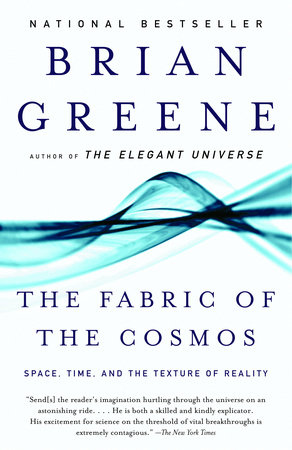
\includegraphics[width=\linewidth]{images/fabric_of_the_cosmos.jpg}
   \varcaption{\href{https://www.penguinrandomhouse.com/books/71273/the-fabric-of-the-cosmos-by-brian-greene/9780375727207/}{Publisher Link}, \href{https://www.amazon.com/Fabric-Cosmos-Space-Texture-Reality/dp/0375727205}{Amazon Link}}
\end{marginfigure}

\begin{itemize}
    \item[] \textbf{Author:} Brian Greene
    \item[] \textbf{Published Year:} 2005
    \item[] \textbf{Publisher:} Penguin Random House/Vintage
    \item[] \textbf{Number of Pages:} 592
    \item[] \textbf{ISBN:} 9780375727207
    \item[] \textbf{Description:} Space and time form the very fabric of the cosmos. Yet they remain among the most mysterious of concepts. Is space an entity? Why does time have a direction? Could the universe exist without space and time? Can we travel to the past? Greene has set himself a daunting task: to explain non-intuitive, mathematical concepts like String Theory, the Heisenberg Uncertainty Principle, and Inflationary Cosmology with analogies drawn from common experience. From Newton’s unchanging realm in which space and time are absolute, to Einstein’s fluid conception of spacetime, to quantum mechanics’ entangled arena where vastly distant objects can instantaneously coordinate their behavior, Greene takes us all, regardless of our scientific backgrounds, on an irresistible and revelatory journey to the new layers of reality that modern physics has discovered lying just beneath the surface of our everyday world.
\end{itemize}

\section*{The C. S. Lewis Signature Classics An Anthology of 8 C. S. Lewis Titles: Mere Christianity, The Screwtape Letters, Miracles, \newline The Great Divorce, The Problem of Pain, A Grief Observed, \newline The Abolition of Man, and The Four Loves}
\begin{marginfigure}[8\baselineskip]
   
\includegraphics[width=\linewidth]{images/cs_lewis.jpg}
   \varcaption{\href{https://www.harpercollins.com/9780062572547/the-c-s-lewis-signature-classics/}{Publisher Link}, \href{https://www.amazon.com/gp/product/0062572547}{Amazon Link}}
\end{marginfigure}

\begin{itemize}
    \item[] \textbf{Author:} C. S. Lewis
    \item[] \textbf{Published Year:} 2017
    \item[] \textbf{Publisher:} Harper Collins/HarperOne
    \item[] \textbf{Number of Pages:} 864
    \item[] \textbf{ISBN:} 9780062572547
    \item[] \textbf{Description:} Available for the first time in one deluxe paperback edition, all eight volumes of the C. S. Lewis Signature Classics. Brought together in one volume, here are the signature spiritual works of one of the most celebrated literary figures of our time. This magnificent compendium includes: \textit{Mere Christianity; The Screwtape Letters; The Great Divorce; The Problem of Pain; Miracles; A Grief Observed; Abolition of Man; The Four Loves.}
\end{itemize}

\section*{Mogworld}
\begin{marginfigure}[5\baselineskip]
   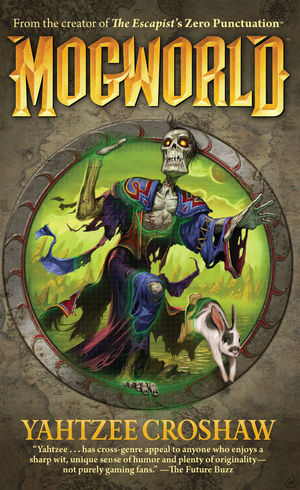
\includegraphics[width=\linewidth]{images/mogworld.jpg}
   \varcaption{\href{https://www.darkhorse.com/Books/16-577/Mogworld}{Publisher Link}, \href{https://www.amazon.com/Mogworld-Yahtzee-Croshaw/dp/1506706355/}{Amazon Link}}
\end{marginfigure}

\begin{itemize}
    \item[] \textbf{Author:} Yahtzee Croshaw
    \item[] \textbf{Published Year:} 2010
    \item[] \textbf{Publisher:} Dark Horse Books
    \item[] \textbf{Number of Pages:} 350
    \item[] \textbf{ISBN:} 9781506706351
    \item[] \textbf{Description:} In a world full to bursting with would-be heroes, Jim couldn't be less interested in saving the day. His fireballs fizzle. He's awfully grumpy. Plus, he's been dead for about sixty years. When a renegade necromancer wrenches him from eternal slumber and into a world gone terribly, bizarrely wrong, all Jim wants is to find a way to die properly, once and for all. On his side, he's got a few shambling corpses, an inept thief, and a powerful death wish. But he's up against tough odds: angry mobs of adventurers, a body falling apart at the seams --- and a team of programmers racing a deadline to hammer out the last few bugs in their AI.
\end{itemize}

\section*{John Dies at the End (John and Dave: Book 1)}
\begin{marginfigure}[3\baselineskip]
   
\includegraphics[width=\linewidth]{images/john_dies_at_the_end.jpg}
   \varcaption{\href{https://us.macmillan.com/books/9780312659141}{Publisher Link}, \href{https://www.amazon.com/John-Dies-End-David-Wong/dp/1250035953}{Amazon Link}}
\end{marginfigure}

\begin{itemize}
    \item[] \textbf{Author:} David Wong
    \item[] \textbf{Published Year:} 2010
    \item[] \textbf{Publisher:} Macmillan/St. Martin's Griffin
    \item[] \textbf{Number of Pages:} 480
    \item[] \textbf{ISBN:} 9780312659141
    \item[] \textbf{Description:} \textbf{STOP.} You should not have touched this book with your bare hands. NO, don't put it down. It's too late. They're watching you. My name is David Wong. My best friend is John. Those names are fake. You might want to change yours. You may not want to know about the things you'll read on these pages, about \textbf{the sauce}, about \textbf{Korrok}, about the invasion, and the future. But it's too late. You touched the book. You're in the game. You're under \textbf{the eye}. The only defense is knowledge. You need to read this book, to the end. Even the part with the bratwurst. Why? You just have to trust me. \textbf{The important thing is this:} The drug is called \textbf{Soy Sauce} and it gives users a window into another dimension. John and I never had the chance to say no. You still do. Unfortunately for us, if you make the right choice, we'll have a much harder time explaining how to \textbf{fight off the otherworldly invasion} currently threatening to \textbf{enslave humanity}. I'm sorry to have involved you in this, I really am. But as you read about these terrible events and the very \textbf{dark epoch} the world is about to enter as a result, it is crucial you keep one thing in mind: \textbf{None of this is was my fault.}
\end{itemize}

\section*{Cryptonomicon}
\begin{marginfigure}[14\baselineskip]
   
\includegraphics[width=\linewidth]{images/cryptonomicon.jpg}
   \varcaption{\href{https://www.harpercollins.com/9780380788620/cryptonomicon/}{Publisher Link}, \href{https://www.amazon.com/Cryptonomicon-Neal-Stephenson/dp/0380788624/}{Amazon Link}}
\end{marginfigure}

\begin{itemize}
    \item[] \textbf{Author:} Neal Stephenson
    \item[] \textbf{Published Year:} 2000
    \item[] \textbf{Publisher:} Harper Collins/William Morrow
    \item[] \textbf{Number of Pages:} 928
    \item[] \textbf{ISBN:} 9780380788620
    \item[] \textbf{Description:} In 1942, Lawrence Pritchard Waterhouse --- mathematical genius and young Captain in the U.S. Navy --- is assigned to detachment 2702. It is an outfit so secret that only a handful of people know it exists, and some of those people have names like Churchill and Roosevelt. The mission of Waterhouse and Detachment 2702 --- commanded by Marine Raider Bobby Shaftoe-is to keep the Nazis ignorant of the fact that Allied Intelligence has cracked the enemy's fabled Enigma code. It is a game, a cryptographic chess match between Waterhouse and his German counterpart, translated into action by the gung-ho Shaftoe and his forces. Fast-forward to the present, where Waterhouse's crypto-hacker grandson, Randy, is attempting to create a "data haven" in Southeast Asia --- a place where encrypted data can be stored and exchanged free of repression and scrutiny. As governments and multinationals attack the endeavor, Randy joins forces with Shaftoe's tough-as-nails granddaughter, Amy, to secretly salvage a sunken Nazi submarine that holds the key to keeping the dream of a data haven afloat. But soon their scheme brings to light a massive conspiracy with its roots in Detachment 2702 linked to an unbreakable Nazi code called Arethusa. And it will represent the path to unimaginable riches and a future of personal and digital liberty\ldots or to universal totalitarianism reborn.
\end{itemize}

\section*{Neuromancer (Sprawl Trilogy: Book 1)}

\begin{marginfigure}[\baselineskip]
   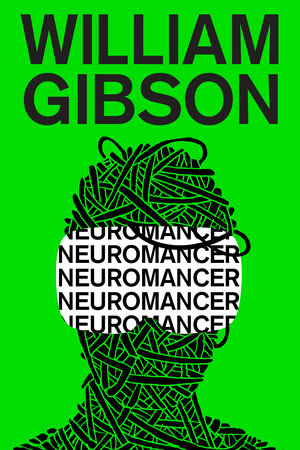
\includegraphics[width=\linewidth]{images/neuromancer.jpg}
   \varcaption{\href{https://www.penguinrandomhouse.com/books/293994/neuromancer-by-william-gibson/9780441007462/}{Publisher Link}, \href{https://www.amazon.com/Neuromancer-William-Gibson/dp/0441569595/}{Amazon Link}}
\end{marginfigure}

\begin{itemize}
    \item[] \textbf{Author:} William Gibson
    \item[] \textbf{Published Year:} 1986
    \item[] \textbf{Publisher:} Penguin Random House/Ace
    \item[] \textbf{Number of Pages:} 336 
    \item[] \textbf{ISBN:} 9780441569595
    \item[] \textbf{Description:} Case was the sharpest data-thief in the matrix --- until he crossed the wrong people and they crippled his nervous system, banishing him from cyberspace. Now a mysterious new employer has recruited him for a last-chance run at an unthinkably powerful artificial intelligence. With a dead man riding shotgun and Molly, a mirror-eyed street-samurai, to watch his back, Case is ready for the adventure that upped the ante on an entire genre of fiction.
\end{itemize}


\section*{Spirits of Place}
\begin{marginfigure}[\baselineskip]
   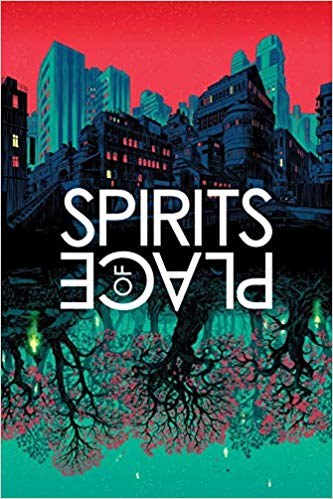
\includegraphics[width=\linewidth]{images/spirits_of_place.jpg}
   \varcaption{\href{https://www.dailygrail.com/2016/12/spirits-of-place-featuring-alan-moore-warren-ellis-and-many-more/}{Publisher Link}, \href{https://www.amazon.com/Spirits-Place-Alan-Moore/dp/0994617631/}{Amazon Link}}
\end{marginfigure}

\begin{itemize}
    \item[] \textbf{Author:} Alan Moore, Warren Ellis, \& John Reppion
    \item[] \textbf{Published Year:} 2016
    \item[] \textbf{Publisher:} Daily Grail
    \item[] \textbf{Number of Pages:} 306
    \item[] \textbf{ISBN:} 9780994617637
    \item[] \textbf{Description:} Stories are embedded in the world around us; in metal, in brick, in concrete, and in wood. In the very earth beneath our feet. Our history surrounds us and the tales we tell, true or otherwise, are always rooted in what has gone before. The spirits of place are the echoes of people, of events, of ideas which have become imprinted upon a location, for better or for worse. They are the \textit{genii loci} of classical Roman religion, the disquieting atmosphere of a former battlefield, the comfort and familiarity of a childhood home. Twelve authors take us on a journey; a tour of places where they themselves have encountered, and consulted with, these \textit{Spirits of Place}.
\end{itemize}

\section*{The Language of Kindness: A Nurse's Story}

\begin{itemize}
    \item[] \textbf{Author:} Christie Watson
    \item[] \textbf{Published Year:} 2019 
    \item[] \textbf{Publisher:} Penguin Random House/Tim Duggan
    \item[] \textbf{Number of Pages:} 336 
    \item[] \textbf{ISBN:} 9781524761646
    \item[] \textbf{Description:} In the neonatal unit, premature babies fight for their lives, hovering at the very edge of survival, like tiny Emmanuel, wrapped up in a sandwich bag. On the cancer wards, the nurses administer chemotherapy and, long after the medicine stops working, something more important --- which Watson learns to recognize when her own father is dying of cancer. In the pediatric intensive care unit, the nurses wash the hair of a little girl to remove the smell of smoke from the house fire. The emergency room is overcrowded as ever, with waves of alcohol and drug addicted patients as well as patients like Betty, a widow suffering chest pain, frail and alone. And the stories of the geriatric ward–Gladys and older patients like her --- show the plight of the most vulnerable members of our society.

\begin{marginfigure}[-23\baselineskip]
   
\includegraphics[width=\linewidth]{images/nurses_story.jpg}
   \varcaption{\href{https://www.penguinrandomhouse.com/books/557756/the-language-of-kindness-by-christie-watson/}{Publisher Link}, \href{https://www.amazon.com/Language-Kindness-Nurses-Story/dp/1524761648/}{Amazon Link}}
\end{marginfigure}

\end{itemize}

\section*{The Monopolists: Obsession, Fury, and the Scandal \newline Behind the World's Favorite Board Game}
\begin{marginfigure}[\baselineskip]
   
\includegraphics[width=\linewidth]{images/monopolists.jpg}
   \varcaption{\href{https://www.bloomsbury.com/us/the-monopolists-9781608199655/}{Publisher Link}, \href{https://www.amazon.com/Monopolists-Obsession-Scandal-Behind-Favorite/dp/1608199657/}{Amazon Link}}
\end{marginfigure}

\begin{itemize}
    \item[] \textbf{Author:} Mary Pilon
    \item[] \textbf{Published Year:} 2016
    \item[] \textbf{Publisher:} Bloomsbury/Bloomsbury USA
    \item[] \textbf{Number of Pages:} 336
    \item[] \textbf{ISBN:} 9781608199655
    \item[] \textbf{Description:} Most think it was invented by an unemployed Pennsylvanian who sold his game to Parker Brothers during the Great Depression in 1935 and lived happily --- and richly --- ever after. That story, however, is not exactly true. Ralph Anspach, a professor fighting to sell his Anti-Monopoly board game decades later, unearthed the real story, which traces back to Abraham Lincoln, the Quakers, and a forgotten feminist named Lizzie Magie who invented her nearly identical Landlord's Game more than thirty years before Parker Brothers sold their version of Monopoly. Her game --- underpinned by morals that were the exact opposite of what Monopoly represents today --- was embraced by a constellation of left-wingers from the Progressive Era through the Great Depression, including members of Franklin Roosevelt's famed Brain Trust.
\end{itemize}

\section*{Sacred Trash: The Lost and Found World of the Cairo Geniza}
\begin{itemize}
    \item[] \textbf{Author:} Adina Hoffman \& Peter Cole
    \item[] \textbf{Published Year:} 2016
    \item[] \textbf{Publisher:} Penguin Random House/Schocken
    \item[] \textbf{Number of Pages:} 304 
    \item[] \textbf{ISBN:} 9780805212235
    \item[] \textbf{Description:} This tale of buried communal treasure weaves together unforgettable portraits of Solomon Schechter and the other modern heroes responsible for the collection’s rescue with explorations of the medieval documents themselves --- letters and poems, wills and marriage contracts, Bibles, money orders, fiery dissenting religious tracts, fashion-conscious trousseaux lists, prescriptions, petitions, and mysterious magical charms. Presenting a pan­oramic view of almost a thousand years of vibrant Mediterranean Judaism, Adina Hoffman and Peter Cole bring contemporary readers into the heart of this little-known trove, whose contents have rightly been dubbed “the Living Sea Scrolls.” Part biography, part meditation on the supreme value the Jewish people has long placed in the written word, Sacred Trash is above all a gripping tale of adventure and redemption. 
\end{itemize}

\begin{marginfigure}[-35\baselineskip]
   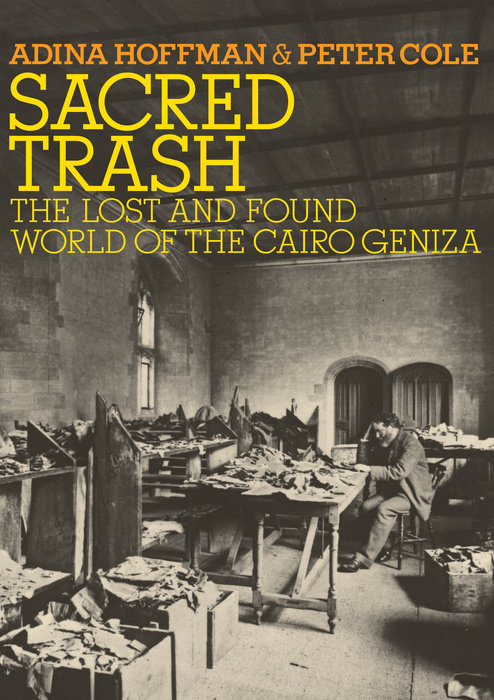
\includegraphics[width=\linewidth]{images/sacred_trash.jpg}
   \varcaption{\href{https://www.penguinrandomhouse.com/books/81238/sacred-trash-by-adina-hoffman-and-peter-cole/}{Publisher Link}, \href{https://www.amazon.com/Sacred-Trash-Geniza-Jewish-Encounters/dp/080521223X/}{Amazon Link}}
\end{marginfigure}

\section*{Toms River: A Story of Science and Salvation}
\begin{marginfigure}[\baselineskip]
   
\includegraphics[width=\linewidth]{images/toms_river.jpg}
   \varcaption{\href{https://islandpress.org/books/toms-river}{Publisher Link}, \href{https://www.amazon.com/Toms-River-Story-Science-Salvation/dp/1610915917/}{Amazon Link}}
\end{marginfigure}

\begin{itemize}
    \item[] \textbf{Author:} Dan Fagin
    \item[] \textbf{Published Year:} 2015
    \item[] \textbf{Publisher:} Island Press
    \item[] \textbf{Number of Pages:} 576 
    \item[] \textbf{ISBN:} 9781610915915
    \item[] \textbf{Description:} One of New Jersey’s seemingly innumerable quiet seaside towns, Toms River became the unlikely setting for a decades-long drama that culminated in 2001 with one of the largest environmental legal settlements in history. For years, large chemical companies had been using Toms River as their private dumping ground, burying tens of thousands of leaky drums in open pits and discharging billions of gallons of acid-laced wastewater into the town’s namesake river. The result was a notorious cluster of childhood cancers scientifically linked to local air and water pollution.
\end{itemize}

\section*{The Faithful Executioner: Life and Death, Honor and Shame in the Turbulent Sixteenth Century}
\begin{marginfigure}[\baselineskip]
   
\includegraphics[width=\linewidth]{images/faithful_executioner.jpg}
   \varcaption{\href{https://us.macmillan.com/books/9781250043610}{Publisher Link}, \href{https://www.amazon.com/Faithful-Executioner-Turbulent-Sixteenth-Century/dp/1250043611/}{Amazon Link}}
\end{marginfigure}

\begin{itemize}
    \item[] \textbf{Author:} Joel F. Harrington
    \item[] \textbf{Published Year:} 2013
    \item[] \textbf{Publisher:} Macmillan/Picador
    \item[] \textbf{Number of Pages:} 320 
    \item[] \textbf{ISBN:} 9781250043610
    \item[] \textbf{Description:} In \textit{The Faithful Executioner}, Harrington teases out the hidden meanings and drama of Schmidt's journal. Deemed an official outcast, Meister Frantz sought to prove himself worthy of honor and free his children from the stigma of his profession. Harrington uncovers details of Schmidt's life and work: the shocking, but often familiar, crimes of the day; the medical practice that he felt was his true calling; and his lifelong struggle to reconcile his craft with his religious faith.
\end{itemize}

\section*{Spook: Science Tackles the Afterlife}
\begin{marginfigure}[3\baselineskip]
   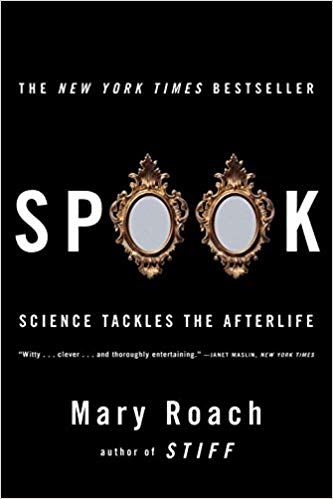
\includegraphics[width=\linewidth]{images/spook.jpg}
   \varcaption{\href{https://wwnorton.com/books/9780393329124}{Publisher Link}, \href{https://www.amazon.com/Spook-Science-Afterlife-Mary-Roach/dp/0393329127/}{Amazon Link}}
\end{marginfigure}

\begin{itemize}
    \item[] \textbf{Author:} Mary Roach
    \item[] \textbf{Published Year:} 2006
    \item[] \textbf{Publisher:} W. W. Norton \& Company
    \item[] \textbf{Number of Pages:} 311  
    \item[] \textbf{ISBN:} 9780393329124
    \item[] \textbf{Description:} ``What happens when we die? Does the light just go out and that's that—the million-year nap? Or will some part of my personality, my me-ness persist? What will that feel like? What will I do all day? Is there a place to plug in my lap-top?'' In an attempt to find out, Mary Roach brings her tireless curiosity to bear on an array of contemporary and historical soul-searchers: scientists, schemers, engineers, mediums, all trying to prove (or disprove) that life goes on after we die.
\end{itemize}

\section*{Ninety Percent of Everything: Inside Shipping, the Invisible Industry That Puts Clothes on Your Back, Gas in Your Car, and Food on Your Plate}

\begin{itemize}
    \item[] \textbf{Author:} Rose George
    \item[] \textbf{Published Year:} 2014
    \item[] \textbf{Publisher:} Macmillan/Picador
    \item[] \textbf{Number of Pages:} 304  
    \item[] \textbf{ISBN:} 9781250058294
    \item[] \textbf{Description:} On ship-tracking Web sites, the waters are black with dots. Each dot is a ship; each ship is laden with boxes; each box is laden with goods. In postindustrial economies, we no longer produce but buy, and so we must ship. Without shipping there would be no clothes, food, paper, or fuel. Without all those dots, the world would not work. Yet freight shipping is all but invisible. Away from public scrutiny, it revels in suspect practices, dubious operators, and a shady system of ``flags of convenience''. And then there are the pirates. Rose George, acclaimed chronicler of what we would rather ignore, sails from Rotterdam to Suez to Singapore on ships the length of football fields and the height of Niagara Falls; she patrols the Indian Ocean with an anti-piracy task force; she joins seafaring chaplains, and investigates the harm that ships inflict on endangered whales. Sharply informative and entertaining, \textit{Ninety Percent of Everything} reveals the workings and perils of an unseen world that holds the key to our economy, our environment, and our very civilization.
\end{itemize}

\begin{marginfigure}[-43\baselineskip]
   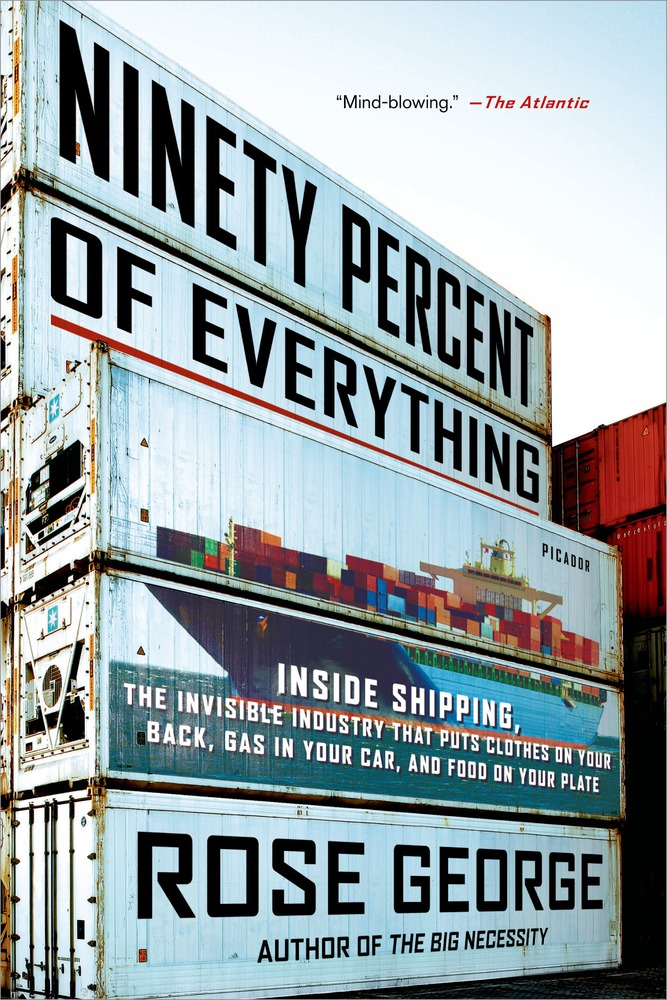
\includegraphics[width=\linewidth]{images/ninety_percent_of_everything.jpg}
   \varcaption{\href{https://us.macmillan.com/books/9781250058294}{Publisher Link}, \href{https://www.amazon.com/Ninety-Percent-Everything-Shipping-Invisible/dp/1250058295/}{Amazon Link}}
\end{marginfigure}

\section*{Animals Strike Curious Poses}
\begin{marginfigure}[1\baselineskip]
   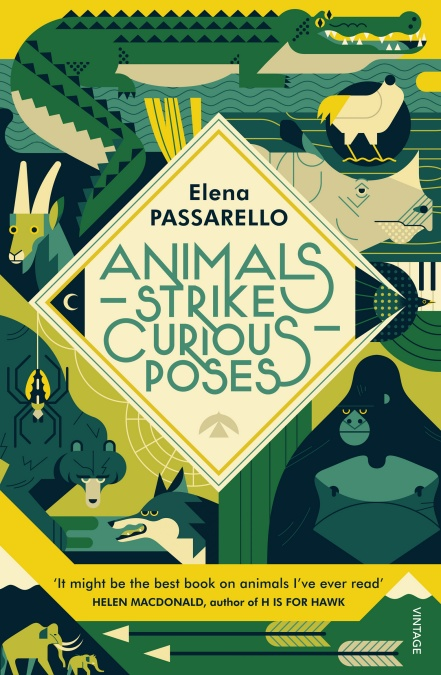
\includegraphics[width=\linewidth]{images/animals_strike_curious_poses.jpg}
   \varcaption{\href{https://www.penguin.co.uk/books/111/1114747/animals-strike-curious-poses/9781784707354.html}{Publisher Link}, \href{https://www.amazon.com/Animals-Strike-Curious-Passarello-author/dp/178470735X/}{Amazon Link}}
\end{marginfigure}

\begin{itemize}
    \item[] \textbf{Author:} Elena Passarello
    \item[] \textbf{Published Year:} 2018
    \item[] \textbf{Publisher:} Penguin UK/Vintage
    \item[] \textbf{Number of Pages:} 256  
    \item[] \textbf{ISBN:} 9781784707354
    \item[] \textbf{Description:} Beginning with Yuka, a 39,000-year-old mummified woolly mammoth recently found in the Siberian permafrost, each of the sixteen essays in \textit{Animals Strike Curious Poses} investigates a different famous animal named and immortalised by humans. Here are the starling that inspired Mozart with its song, Darwin’s tortoise Harriet, and in an extraordinary essay, Jumbo the elephant (and how they tried to electrocute him). Modelled loosely on a medieval bestiary, these witty , playful, provocative essays traverse history, myth, science and more, introducing a stunning new writer to British readers.
\end{itemize}

\section*{Word by Word: The Secret Life of Dictionaries}
\begin{marginfigure}[\baselineskip]
   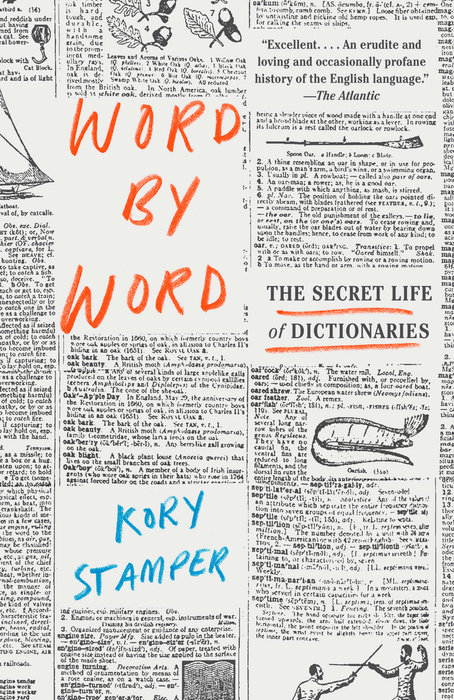
\includegraphics[width=\linewidth]{images/word_by_word.jpg}
   \varcaption{\href{https://www.penguinrandomhouse.com/books/530504/word-by-word-by-kory-stamper/}{Publisher Link}, \href{https://www.amazon.com/Word-Secret-Life-Dictionaries/dp/110197026X/}{Amazon Link}}
\end{marginfigure}

\begin{itemize}
    \item[] \textbf{Author:} Kory Stamper
    \item[] \textbf{Published Year:} 2018
    \item[] \textbf{Publisher:} Penguin Random House/Vintage
    \item[] \textbf{Number of Pages:} 320   
    \item[] \textbf{ISBN:} 9781101970263
    \item[] \textbf{Description:} With wit and irreverence, lexicographer Kory Stamper cracks open the obsessive world of dictionary writing, from the agonizing decisions about what to define and how to do it to the knotty questions of ever-changing word usage. Filled with fun facts --- for example, the first documented usage of ``OMG'' was in a letter to Winston Churchill --- and Stamper’s own stories from the linguistic front lines (including how she became America’s foremost ``irregardless'' apologist, despite loathing the word), \textit{Word by Word} is an endlessly entertaining look at the wonderful complexities and eccentricities of the English language.
\end{itemize}

\section*{Ghostland: An American History in Haunted Places}
\begin{marginfigure}[4\baselineskip]
   
\includegraphics[width=\linewidth]{images/ghostland.jpg}
   \varcaption{\href{https://www.penguinrandomhouse.com/books/531470/ghostland-by-colin-dickey/9781101980200/}{Publisher Link}, \href{https://www.amazon.com/gp/product/1101980206/}{Amazon Link}}
\end{marginfigure}

\begin{itemize}
    \item[] \textbf{Author:} Colin Dickey
    \item[] \textbf{Published Year:} 2017
    \item[] \textbf{Publisher:} Penguin Random House/Penguin
    \item[] \textbf{Number of Pages:} 336   
    \item[] \textbf{ISBN:} 9781101980200
    \item[] \textbf{Description:} Colin Dickey is on the trail of America’s ghosts. Crammed into old houses and hotels, abandoned prisons and empty hospitals, the spirits that linger continue to capture our collective imagination, but why? His own fascination piqued by a house hunt in Los Angeles that revealed derelict foreclosures and ``zombie homes,'', Dickey embarks on a journey across the continental United States to decode and unpack the American history repressed in our most famous haunted places. Some have established reputations as ``the most haunted mansion in America,'' or ``the most haunted prison''; others, like the haunted Indian burial grounds in West Virginia, evoke memories from the past our collective nation tries to forget. With boundless curiosity, Dickey conjures the dead by focusing on questions of the living --- how do we, the living, deal with stories about ghosts, and how do we inhabit and move through spaces that have been deemed, for whatever reason, haunted? Paying attention not only to the true facts behind a ghost story, but also to the ways in which changes to those facts are made --- and why those changes are made --- Dickey paints a version of American history left out of the textbooks, one of things left undone, crimes left unsolved.
\end{itemize}

\section*{The Dragon Behind the Glass: A True Story of Power, Obsession, and the World's Most Coveted Fish}
\begin{marginfigure}[10\baselineskip]
   
\includegraphics[width=\linewidth]{images/dragon_behind_the_glass.jpg}
   \varcaption{\href{https://www.simonandschuster.com/books/The-Dragon-Behind-the-Glass/Emily-Voigt/9781451678949}{Publisher Link}, \href{https://www.amazon.com/Dragon-Behind-Glass-Obsession-Coveted/dp/1451678959/}{Amazon Link}}
\end{marginfigure}

\begin{itemize}
    \item[] \textbf{Author:} Emily Voigt
    \item[] \textbf{Published Year:} 2016
    \item[] \textbf{Publisher:} Simon \& Schuster/Scribner
    \item[] \textbf{Number of Pages:} 336   
    \item[] \textbf{ISBN:} 9781451678949
    \item[] \textbf{Description:} A young man is murdered for his prized pet fish. An Asian tycoon buys a single specimen for \$150,000. Meanwhile, a pet detective chases smugglers through the streets of New York. Delving into an outlandish realm of obsession, paranoia, and criminality, The Dragon Behind the Glass tells the story of a fish like none other: a powerful predator dating to the age of the dinosaurs. Treasured as a status symbol believed to bring good luck, the Asian arowana is bred on high-security farms in Southeast Asia and sold by the hundreds of thousands each year. In the United States, however, it’s protected by the Endangered Species Act and illegal to bring into the country --- though it remains the object of a thriving black market. From the South Bronx to Singapore, journalist Emily Voigt follows the trail of the fish, ultimately embarking on a years-long quest to find the arowana in the wild, venturing deep into some of the last remaining tropical wildernesses on earth.
\end{itemize}

\section*{Rare Books Uncovered: True Stories of Fantastic Finds in Unlikely Places}

\begin{itemize}
    \item[] \textbf{Author:} Rebecca Rego Barry
    \item[] \textbf{Published Year:} 2018
    \item[] \textbf{Publisher:} Quarto/Voyageur
    \item[] \textbf{Number of Pages:} 280   
    \item[] \textbf{ISBN:} 9780760361573
    \item[] \textbf{Description:} Few collectors are as passionate or as dogged in the pursuit of their quarry as collectors of rare books. In Rare Books Uncovered, expert on rare and antiquarian books Rebecca Rego Barry recounts the stories of remarkable discoveries from the world of book collecting. Read about the family whose discovery in their attic of a copy of Action Comics No. 1 --- the first appearance of Superman --- saved their home from foreclosure. Or the Salt Lake City bookseller who volunteered for a local fundraiser --- and came across a 500-year-old copy of the Nuremberg Chronicle. Or the collector who, while browsing his local thrift shop, found a collectible copy of Calvary in China --- inscribed by the author to the collector's grandfather. These tales and many others will entertain and inspire casual collectors and hardcore bibliomaniacs alike.
\end{itemize}

\begin{marginfigure}[-22\baselineskip]
   
\includegraphics[width=\linewidth]{images/rare_books.jpg}
   \varcaption{\href{https://www.quartoknows.com/books/9780760361573/Rare-Books-Uncovered.html}{Publisher Link}, \href{https://www.amazon.com/Rare-Books-Uncovered-Fantastic-Unlikely/dp/0760361576/}{Amazon Link}}
\end{marginfigure}

\section*{The Hunt for Vulcan: \ldots and How Albert Einstein Destroyed \newline a Planet, Discovered Relativity, and Deciphered the Universe}
\begin{marginfigure}[\baselineskip]
   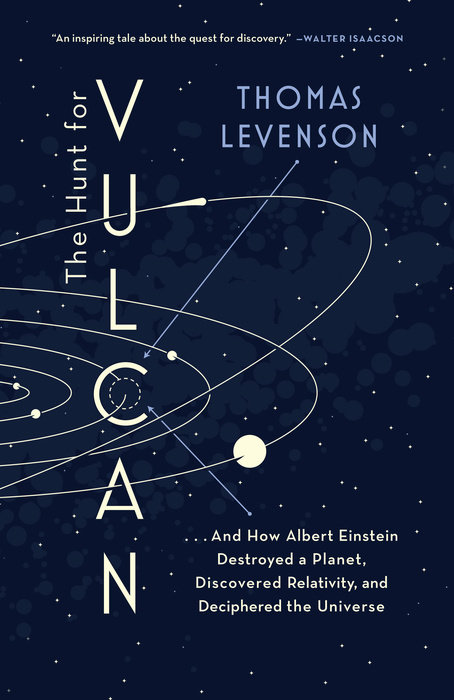
\includegraphics[width=\linewidth]{images/hunt_for_vulcan.jpg}
   \varcaption{\href{https://www.penguinrandomhouse.com/books/254788/the-hunt-for-vulcan-by-thomas-levenson/9780812988307/}{Publisher Link}, \href{https://www.amazon.com/Hunt-Vulcan-Discovered-Relativity-Deciphered/dp/0812988302/}{Amazon Link}}
\end{marginfigure}

\begin{itemize}
    \item[] \textbf{Author:} Thomas Levenson
    \item[] \textbf{Published Year:} 2016
    \item[] \textbf{Publisher:} Penguin Random House/Random House
    \item[] \textbf{Number of Pages:} 256    
    \item[] \textbf{ISBN:} 97814597808129883071678949
    \item[] \textbf{Description:} In \textit{The Hunt for Vulcan}, Thomas Levenson follows the visionary scientists who inhabit the story of the phantom planet, starting with Isaac Newton, who in 1687 provided an explanation for all matter in motion throughout the universe, leading to Urbain-Jean-Joseph Le Verrier, who almost two centuries later built on Newton’s theories and discovered Neptune, becoming the most famous scientist in the world. Le Verrier attempted to surpass that triumph by predicting the existence of yet another planet in our solar system, Vulcan. It took Albert Einstein to discern that the mystery of the missing planet was a problem not of measurements or math but of Newton’s theory of gravity itself. Einstein’s general theory of relativity proved that Vulcan did not and could not exist, and that the search for it had merely been a quirk of operating under the wrong set of assumptions about the universe. Levenson tells the previously untold tale of how the “discovery” of Vulcan in the nineteenth century set the stage for Einstein’s monumental breakthrough, the greatest individual intellectual achievement of the twentieth century.
\end{itemize}

\section*{A Wilder Time: Notes from a Geologist at the Edge of the Greenland Ice}
\begin{marginfigure}[5\baselineskip]
   
\includegraphics[width=\linewidth]{images/wilder_time.jpg}
   \varcaption{\href{https://blpress.org/books/a-wilder-time/}{Publisher Link}, \href{https://www.amazon.com/Wilder-Time-Notes-Geologist-Greenland/dp/1942658346/}{Amazon Link}}
\end{marginfigure}

\begin{itemize}
    \item[] \textbf{Author:} William E. Glassley 
    \item[] \textbf{Published Year:} 2018
    \item[] \textbf{Publisher:} Bellevue Literary Press
    \item[] \textbf{Number of Pages:} 224    
    \item[] \textbf{ISBN:} 9781942658344
    \item[] \textbf{Description:} Greenland, one of the last truly wild places, contains a treasure trove of information on Earth’s early history embedded in its pristine landscape. Over numerous seasons, William E. Glassley and two fellow geologists traveled there to collect samples and observe rock formations for evidence to prove a contested theory that plate tectonics, the movement of Earth’s crust over its molten core, is a much more ancient process than some believed. As their research drove the scientists ever farther into regions barely explored by humans for millennia --- if ever --- Glassley encountered wondrous creatures and natural phenomena that gave him unexpected insight into the origins of myth, the virtues and boundaries of science, and the importance of seeking the wilderness within.
\end{itemize}

\section*{Mammother}
\begin{marginfigure}[10\baselineskip]
   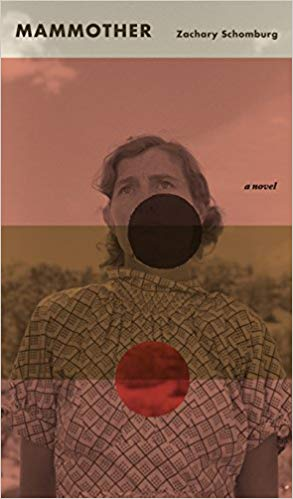
\includegraphics[width=\linewidth]{images/mammother.jpg}
   \varcaption{\href{http://www.featherproof.com/catalog/mammother}{Publisher Link}, \href{https://www.amazon.com/Mammother-Zachary-Schomburg/dp/1943888108/}{Amazon Link}}
\end{marginfigure}

\begin{itemize}
    \item[] \textbf{Author:} Zachary Schomburg 
    \item[] \textbf{Published Year:} 2017
    \item[] \textbf{Publisher:} Featherproof
    \item[] \textbf{Number of Pages:} 328    
    \item[] \textbf{ISBN:} 9781943888108
    \item[] \textbf{Description:} In \textit{Mammother}, the people of Pie Time are suffering from God’s Finger, a mysterious plague that leaves its victims dead with a big hole through their chests, and in each hole is a random consumer product. Mano Medium is a sensitive, young cigarette-factory worker in love, and he does his part by quitting the factory to work double-time as Pie Time’s replacement barber and butcher, and by holding the things found in the holes of the newly dead. However, the more people die, the bigger Mano becomes. Elsewhere in Pie Time, XO (the power-hungry corporation bent on overtaking Pie Time) and Father Mothers (the bumbling priest) have their own ideas about how to capitalize on God’s Finger. Mano encourages resistance to their exploitation by teaching death to those who can’t afford to survive it. But as Pie Time and Mano both grow irrevocably, Mano must make a decision about how he can best fit into his own life.
\end{itemize}

\section*{The Woman Who Smashed Codes: A True Story of Love, Spies, and the Unlikely Heroine Who Outwitted America's Enemies}
\begin{marginfigure}[14\baselineskip]
   
\includegraphics[width=\linewidth]{images/woman_who_smashes_codes.jpg}
   \varcaption{\href{https://www.harpercollins.com/9780062430489/the-woman-who-smashed-codes/}{Publisher Link}, \href{https://www.amazon.com/Woman-Who-Smashed-Codes-Outwitted/dp/0062430513/}{Amazon Link}}
\end{marginfigure}

\begin{itemize}
    \item[] \textbf{Author:} Jason Fagone 
    \item[] \textbf{Published Year:} 2018
    \item[] \textbf{Publisher:} Harper Collins/Dey Street
    \item[] \textbf{Number of Pages:} 464    
    \item[] \textbf{ISBN:} 9780062430519
    \item[] \textbf{Description:} In 1916, at the height of World War I, brilliant Shakespeare expert Elizebeth Smith went to work for an eccentric tycoon on his estate outside Chicago. The tycoon had close ties to the U.S. government, and he soon asked Elizebeth to apply her language skills to an exciting new venture: code-breaking. There she met the man who would become her husband, groundbreaking cryptologist William Friedman. Though she and Friedman are in many ways the ``Adam and Eve'' of the NSA, Elizebeth’s story, incredibly, has never been told. In The Woman Who Smashed Codes, Jason Fagone chronicles the life of this extraordinary woman, who played an integral role in our nation’s history for forty years. After World War I, Smith used her talents to catch gangsters and smugglers during Prohibition, then accepted a covert mission to discover and expose Nazi spy rings that were spreading like wildfire across South America, advancing ever closer to the United States. As World War II raged, Elizebeth fought a highly classified battle of wits against Hitler’s Reich, cracking multiple versions of the Enigma machine used by German spies. Meanwhile, inside an Army vault in Washington, William worked furiously to break Purple, the Japanese version of Enigma --- and eventually succeeded, at a terrible cost to his personal life.
\end{itemize}

\section*{Tyrant: Shakespeare on Politics}
\begin{marginfigure}[\baselineskip]
   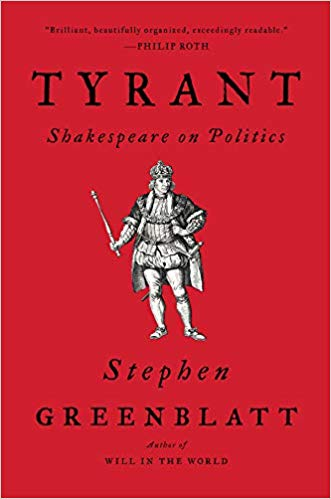
\includegraphics[width=\linewidth]{images/tyrant.jpg}
   \varcaption{\href{https://wwnorton.com/books/9780393356977}{Publisher Link}, \href{https://www.amazon.com/Tyrant-Shakespeare-Politics-Stephen-Greenblatt/dp/0393356973/}{Amazon Link}}
\end{marginfigure}

\begin{itemize}
    \item[] \textbf{Author:} Stephen Greenblatt 
    \item[] \textbf{Published Year:} 2019
    \item[] \textbf{Publisher:} W. W. Norton \& Company
    \item[] \textbf{Number of Pages:} 224    
    \item[] \textbf{ISBN:} 9780393356977
    \item[] \textbf{Description:} Examining the psyche --- and psychoses --- of the likes of Richard III, Macbeth, Lear, and Coriolanus, Greenblatt illuminates the ways in which William Shakespeare delved into the lust for absolute power and the disasters visited upon the societies over which these characters rule. Tyrant shows that Shakespeare’s work remains vitally relevant today, not least in its probing of the unquenchable, narcissistic appetites of demagogues and the self-destructive willingness of collaborators who indulge them.
\end{itemize}

\section*{The Library Book}
\begin{marginfigure}[2\baselineskip]
   
\includegraphics[width=\linewidth]{images/library_book.jpg}
   \varcaption{\href{https://www.simonandschuster.com/books/The-Library-Book/Susan-Orlean/9781476740188}{Publisher Link}, \href{https://www.amazon.com/Library-Book-Susan-Orlean/dp/1476740194/}{Amazon Link}}
\end{marginfigure}

\begin{itemize}
    \item[] \textbf{Author:} Susan Orlean 
    \item[] \textbf{Published Year:} 2019
    \item[] \textbf{Publisher:} Simon \& Schuster
    \item[] \textbf{Number of Pages:} 336    
    \item[] \textbf{ISBN:} 9781476740195
    \item[] \textbf{Description:} On the morning of April 28, 1986, a fire alarm sounded in the Los Angeles Public Library. The fire was disastrous: it reached two thousand degrees and burned for more than seven hours. By the time it was extinguished, it had consumed four hundred thousand books and damaged seven hundred thousand more. Investigators descended on the scene, but more than thirty years later, the mystery remains: Did someone purposefully set fire to the library --- and if so, who? Susan Orlean delivers a delightful reflection on the past, present, and future of libraries in America that manages to tell the broader story of libraries and librarians in a way that has never been done before.
\end{itemize}

\section*{Do No Harm: Stories of Life, Death, and Brain Surgery}

\begin{itemize}
    \item[] \textbf{Author:} Henry Marsh 
    \item[] \textbf{Published Year:} 2016
    \item[] \textbf{Publisher:} Macmillan/Picador
    \item[] \textbf{Number of Pages:} 320    
    \item[] \textbf{ISBN:} 9781250090133
    \item[] \textbf{Description:} What is it like to be a brain surgeon? How does it feel to hold someone’s life in your hands, to cut into the stuff that creates thought, feeling and reason? How do you live with the consequences of performing a potentially lifesaving operation when it all goes wrong? With astonishing compassion and candor, leading neurosurgeon Henry Marsh reveals the fierce joy of operating, the profoundly moving triumphs, the harrowing disasters, the haunting regrets and the moments of black humor that characterize a brain surgeon’s life. Do No Harm provides unforgettable insight into the countless human dramas that take place in a busy modern hospital. Above all, it is a lesson in the need for hope when faced with life’s most difficult decisions.
\end{itemize}

\begin{marginfigure}[-30\baselineskip]
   
\includegraphics[width=\linewidth]{images/do_no_harm.jpg}
   \varcaption{\href{https://us.macmillan.com/books/9781250090133}{Publisher Link}, \href{https://www.amazon.com/Do-No-Harm-Stories-Surgery/dp/125009013X/}{Amazon Link}}
\end{marginfigure}

\section*{Circe}
\begin{marginfigure}[\baselineskip]
   
\includegraphics[width=\linewidth]{images/circe.jpg}
   \varcaption{\href{https://www.littlebrown.com/titles/madeline-miller/circe/9780316556323/}{Publisher Link}, \href{https://www.amazon.com/Circe-Madeline-Miller/dp/0316556327/}{Amazon Link}}
\end{marginfigure}

\begin{itemize}
    \item[] \textbf{Author:} Madeline Miller 
    \item[] \textbf{Published Year:} 2020
    \item[] \textbf{Publisher:} Hachette/Back Bay
    \item[] \textbf{Number of Pages:} 416     
    \item[] \textbf{ISBN:} 9780316556323
    \item[] \textbf{Description:} In the house of Helios, god of the sun and mightiest of the Titans, a daughter is born. But Circe is a strange child--not powerful, like her father, nor viciously alluring like her mother. Turning to the world of mortals for companionship, she discovers that she does possess power --- the power of witchcraft, which can transform rivals into monsters and menace the gods themselves. Threatened, Zeus banishes her to a deserted island, where she hones her occult craft, tames wild beasts and crosses paths with many of the most famous figures in all of mythology, including the Minotaur, Daedalus and his doomed son Icarus, the murderous Medea, and, of course, wily Odysseus. But there is danger, too, for a woman who stands alone, and Circe unwittingly draws the wrath of both men and gods, ultimately finding herself pitted against one of the most terrifying and vengeful of the Olympians. To protect what she loves most, Circe must summon all her strength and choose, once and for all, whether she belongs with the gods she is born from, or the mortals she has come to love.
\end{itemize}

\section*{The Hidden Reality: Parallel Universes and the Deep Laws of the Cosmos}
\begin{marginfigure}[7\baselineskip]
   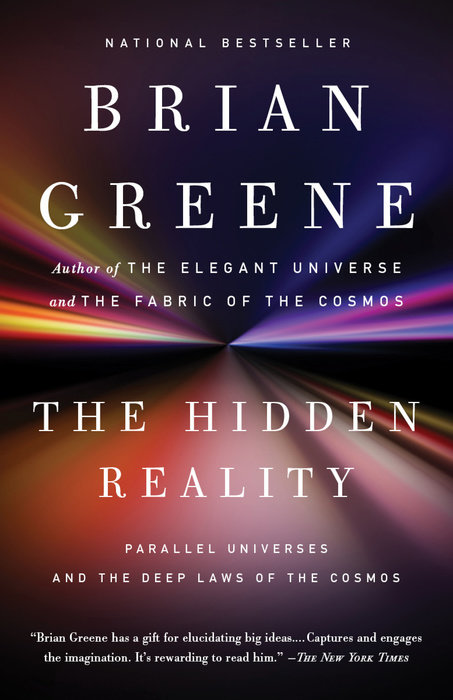
\includegraphics[width=\linewidth]{images/hidden_reality.jpg}
   \varcaption{\href{https://www.penguinrandomhouse.com/books/71272/the-hidden-reality-by-brian-greene/9780307278128/}{Publisher Link}, \href{https://www.amazon.com/Hidden-Reality-Parallel-Universes-Cosmos/dp/0307278123/}{Amazon Link}}
\end{marginfigure}

\begin{itemize}
    \item[] \textbf{Author:} Brian Greene 
    \item[] \textbf{Published Year:} 2011
    \item[] \textbf{Publisher:} Penguin Random House/Vintage
    \item[] \textbf{Number of Pages:} 443      
    \item[] \textbf{ISBN:} 9780307278128
    \item[] \textbf{Description:} There was a time when ``universe'' meant all there is. Everything. Yet, a number of theories are converging on the possibility that our universe may be but one among many parallel universes populating a vast multiverse. Here, Briane Greene, one of our foremost physicists and science writers, takes us on a breathtaking journey to a multiverse comprising an endless series of big bangs, a multiverse with duplicates of every one of us, a multiverse populated by vast sheets of spacetime, a multiverse in which all we consider real are holographic illusions, and even a multiverse made purely of math–and reveals the reality hidden within each.
\end{itemize}

\section*{We Have No Idea: A Guide to the Unknown Universe}
\begin{marginfigure}[8\baselineskip]
   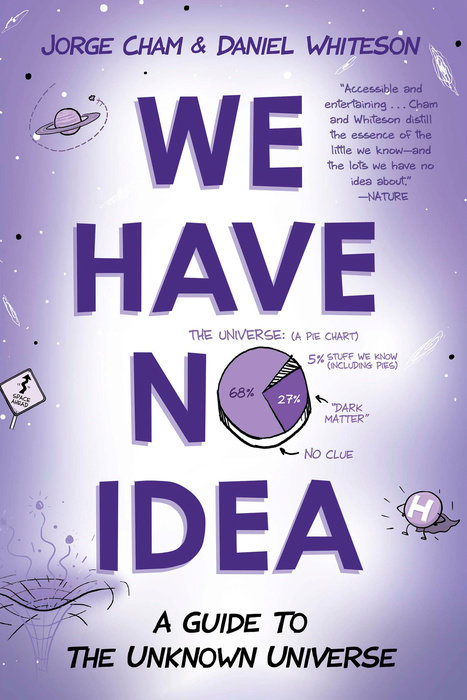
\includegraphics[width=\linewidth]{images/we_have_no_idea.jpg}
   \varcaption{\href{https://www.penguinrandomhouse.com/books/545019/we-have-no-idea-by-jorge-cham-and-daniel-whiteson/}{Publisher Link}, \href{https://www.amazon.com/We-Have-No-Idea-Universe/dp/0735211523/}{Amazon Link}}
\end{marginfigure}

\begin{itemize}
    \item[] \textbf{Author:} Jorge Cham \& Daniel Whiteson 
    \item[] \textbf{Published Year:} 2017
    \item[] \textbf{Publisher:} Penguin Random House/Riverhead
    \item[] \textbf{Number of Pages:} 368      
    \item[] \textbf{ISBN:} 9780735211520
    \item[] \textbf{Description:} Humanity’s understanding of the physical world is full of gaps. Not tiny little gaps you can safely ignore —there are huge yawning voids in our basic notions of how the world works. PHD Comics creator Jorge Cham and particle physicist Daniel Whiteson have teamed up to explore everything we don’t know about the universe: the enormous holes in our knowledge of the cosmos. Armed with their popular infographics, cartoons, and unusually entertaining and lucid explanations of science, they give us the best answers currently available for a lot of questions that are still perplexing scientists. It turns out the universe is full of weird things that don’t make any sense. But Cham and Whiteson make a compelling case that the questions we can’t answer are as interesting as the ones we can.
\end{itemize}

\section*{Soonish: Ten Emerging Technologies That'll Improve and/or Ruin Everything}
\begin{marginfigure}[12\baselineskip]
   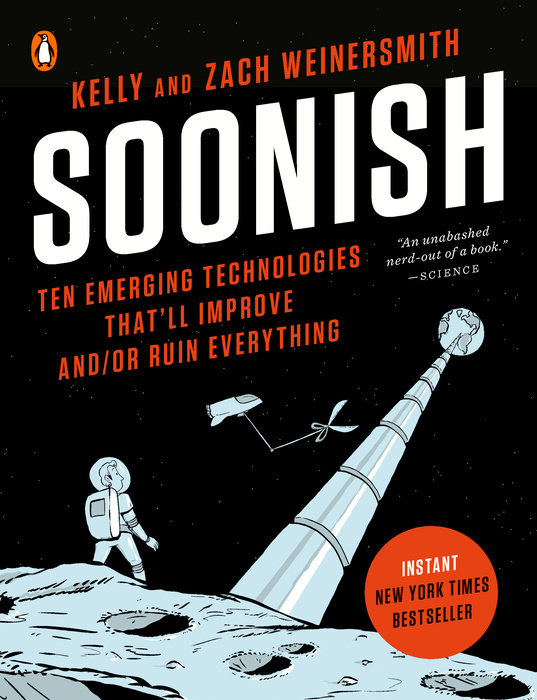
\includegraphics[width=\linewidth]{images/soonish.jpg}
   \varcaption{\href{https://www.penguinrandomhouse.com/books/536910/soonish-by-kelly-and-zach-weinersmith/}{Publisher Link}, \href{https://www.amazon.com/Soonish-Emerging-Technologies-Improve-Everything/dp/0399563849/}{Amazon Link}}
\end{marginfigure}

\begin{itemize}
    \item[] \textbf{Author:} Kelly Weinersmith \& Zach Weinersmith 
    \item[] \textbf{Published Year:} 2019
    \item[] \textbf{Publisher:} Penguin Random House/Penguin
    \item[] \textbf{Number of Pages:} 368      
    \item[] \textbf{ISBN:} 9780399563843
    \item[] \textbf{Description:} What will the world of tomorrow be like? How does progress happen? And why do we not have a lunar colony already? What is the hold-up? In this smart and funny book, celebrated cartoonist Zach Weinersmith and noted researcher Dr. Kelly Weinersmith give us a snapshot of what’s coming next --- from robot swarms to nuclear fusion powered-toasters. By weaving their own research, interviews with the scientists who are making these advances happen, and Zach’s trademark comics, the Weinersmiths investigate why these technologies are needed, how they would work, and what is standing in their way.
\end{itemize}

\section*{The Count of Monte Cristo}
\begin{marginfigure}[9\baselineskip]
   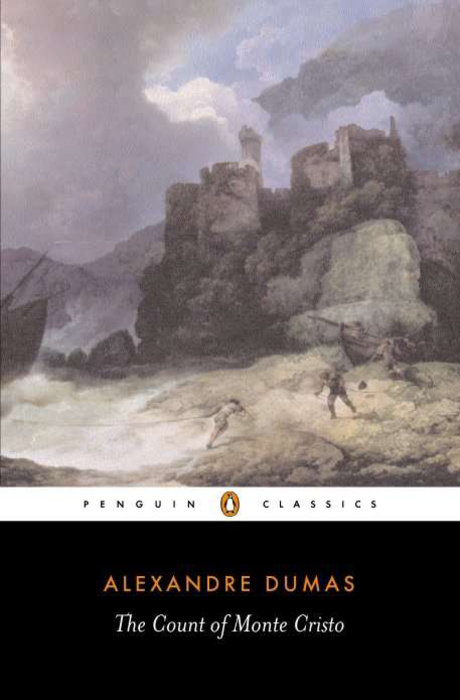
\includegraphics[width=\linewidth]{images/count_of_monte_cristo.jpg}
   \varcaption{\href{https://www.penguinrandomhouse.com/books/286345/the-count-of-monte-cristo-by-alexandre-dumas-pere/}{Publisher Link}, \href{https://www.amazon.com/Count-Monte-Cristo-Penguin-Classics/dp/0140449264/}{Amazon Link}}
\end{marginfigure}

\begin{itemize}
    \item[] \textbf{Author:} Alexandre Dumas père \& Robin Buss
    \item[] \textbf{Published Year:} 2003
    \item[] \textbf{Publisher:} Penguin Random House/Penguin Classics
    \item[] \textbf{Number of Pages:} 1312      
    \item[] \textbf{ISBN:} 9780140449266
    \item[] \textbf{Description:} Thrown in prison for a crime he has not committed, Edmond Dantes is confined to the grim fortress of If. There he learns of a great hoard of treasure hidden on the Isle of Monte Cristo and he becomes determined not only to escape, but also to unearth the treasure and use it to plot the destruction of the three men responsible for his incarceration. Dumas’ epic tale of suffering and retribution, inspired by a real-life case of wrongful imprisonment, was a huge popular success when it was first serialized in the 1840s.
\end{itemize}

\section*{Brock Biology of Microorganisms (Global Edition)}
\begin{marginfigure}[9\baselineskip]
   
\includegraphics[width=\linewidth]{images/brock.jpeg}
   \varcaption{\href{https://www.pearson.com/nl/en_NL/higher-education/subject-catalogue/biology/Brock-Biology-of-Microorganisms-Madigan.html}{Publisher Link}, \href{https://www.amazon.com/Brock-Biology-Microorganisms-Madigan-Michael/dp/1292235101/}{Amazon Link}}
\end{marginfigure}

\begin{itemize}
    \item[] \textbf{Author:} Michael T. Madigan, Kelly S. Bender, Daniel H. Buckley, W. Matthew Sattley, \& David A. Stahl
    \item[] \textbf{Published Year:} 2018
    \item[] \textbf{Publisher:} Pearson
    \item[] \textbf{Number of Pages:} 1064      
    \item[] \textbf{ISBN:} 9781292235103
    \item[] \textbf{Description:} Brock Biology of Microorganisms is the leading majors microbiology text on the market. It sets the standard for impeccable scholarship, accuracy, and strong coverage of ecology, evolution, and metabolism. The 15th edition seamlessly integrates the most current science, paying particular attention to molecular biology and the genomic revolution. It introduces a flexible, more streamlined organization with a consistent level of detail and comprehensive art program.
\end{itemize}

\section*{Lao Tzu: Tao Te Ching --- A Book about the Way and the Power of the Way}
\begin{marginfigure}[9\baselineskip]
   
\includegraphics[width=\linewidth]{images/tao_te_ching.jpg}
   \varcaption{\href{https://www.penguinrandomhouse.com/books/99496/lao-tzu-tao-te-ching-by-ursula-k-le-guin/9781611807240/}{Publisher Link}, \href{https://www.amazon.com/Lao-Tzu-Ching-about-Power/dp/1611807247/}{Amazon Link}}
\end{marginfigure}

\begin{itemize}
    \item[] \textbf{Author:} Lao Tzu, Ursula K. Le Guin
    \item[] \textbf{Published Year:} 2019
    \item[] \textbf{Publisher:} Penguin Random House/Shambhala
    \item[] \textbf{Number of Pages:} 136      
    \item[] \textbf{ISBN:} 9781611807240
    \item[] \textbf{Description:} A rich, poetic, and socially relevant version of the great spiritual and philosophical classic of Taoism from one of America’s leading literary figures. In this landmark modern-day rendition of the ancient Taoist classic, Ursula K. Le Guin presents Lao Tzu’s time-honored and astonishingly powerful philosophy like never before. Drawing on a lifetime of contemplation and including extensive personal commentary throughout, she offers an unparalleled window into the text’s awe-inspiring, immediately relatable teachings and their inestimable value for our troubled world.
\end{itemize}

\section*{Orsinia}
\begin{marginfigure}[7\baselineskip]
   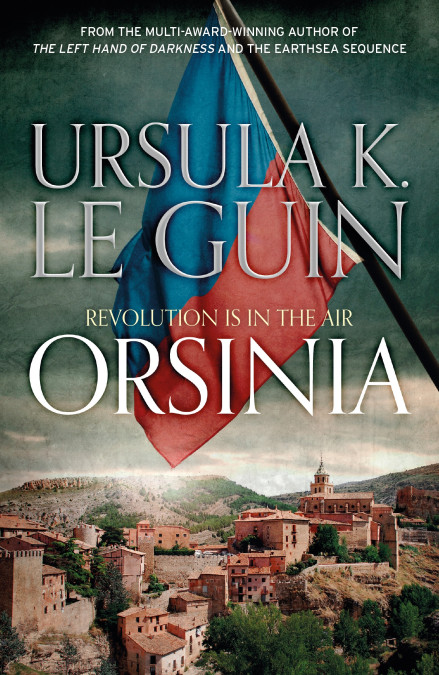
\includegraphics[width=\linewidth]{images/orsinia.jpg}
   \varcaption{\href{https://www.gollancz.co.uk/titles/ursula-k-le-guin/orsinia/9781473212060/}{Publisher Link}, \href{https://www.amazon.com/Orsinia-Malafrena-Orsinian-Fantasy-Masterworks/dp/1473212065/}{Amazon Link}}
\end{marginfigure}

\begin{itemize}
    \item[] \textbf{Author:} Ursula K. Le Guin
    \item[] \textbf{Published Year:} 2017
    \item[] \textbf{Publisher:} Orion/Gollancz
    \item[] \textbf{Number of Pages:} 506      
    \item[] \textbf{ISBN:} 9781473212060
    \item[] \textbf{Description:} Among the less-traveled mountains and plains of Central Europe, a little east of Austria perhaps and north of Slovenia, lies the old kingdom of Orsinia. A land of forests and quiet farmlands and towns, with its capital city Krasnoy on the broad Molsen River, Orsinia has always found itself, like all the countries of Europe, subject to forces beyond its borders. Yet, cast as they are in the shadow of tyrannies both Western and Eastern, the lives and dreams of its free people are no less important than the great arguments of Europe’s emperors and dictators. Here then are those lives: in tales of romance and blood-lust, hope and fear, freedom and tyranny, passion and despair. Tales of love, of life and of death and – amidst the great 19th-century rise of liberalism and nationalism – a tale of revolution against the might of the Hapsburg Empire. This is Orsinia and these are her stories.
\end{itemize}

\section*{Firefall (Blindsight \& Echopraxia)}
\begin{marginfigure}[9\baselineskip]
   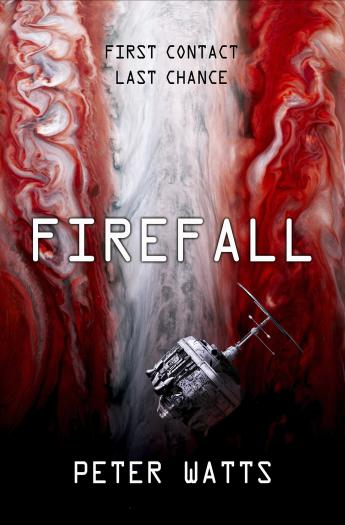
\includegraphics[width=\linewidth]{images/firefall.jpg}
   \varcaption{\href{https://headofzeus.com/books/9781784080457}{Publisher Link}, \href{https://www.amazon.com/Firefall-Peter-Watts-author/dp/178669610X/}{Amazon Link}}
\end{marginfigure}

\begin{itemize}
    \item[] \textbf{Author:} Peter Watts
    \item[] \textbf{Published Year:} 2014
    \item[] \textbf{Publisher:} Head of Zeus
    \item[] \textbf{Number of Pages:} 768      
    \item[] \textbf{ISBN:} 9781784080457
    \item[] \textbf{Description:} February 13, 2082, First Contact. Sixty-two thousand objects of unknown origin plunge into Earth's atmosphere --- a perfect grid of falling stars screaming across the radio spectrum as they burn. Not even ashes reach the ground. Three hundred and sixty degrees of global surveillance: something just took a snapshot. And then\ldots nothing. But from deep space, whispers. Something out there talks – but not to us. Two ships, Theseus and the Crown of Thorns, are launched to discover the origin of Earth's visitation, one bound for the outer dark of the Kuiper Belt, the other for the heart of the Solar System. Their crews can barely be called human, what they will face certainly can't.
\end{itemize}

\section*{Pale Fire}
\begin{marginfigure}[10\baselineskip]
   
\includegraphics[width=\linewidth]{images/pale_fire.jpg}
   \varcaption{\href{https://www.penguinrandomhouse.com/books/119451/pale-fire-by-vladimir-nabokov/9780679410775/}{Publisher Link}, \href{https://www.amazon.com/Pale-Fire-Vladimir-Nabokov/dp/0679723420/}{Amazon Link}}
\end{marginfigure}

\begin{itemize}
    \item[] \textbf{Author:} Vladimir Nabokov
    \item[] \textbf{Published Year:} 1989
    \item[] \textbf{Publisher:} Penguin Random House/Vintage
    \item[] \textbf{Number of Pages:} 320     
    \item[] \textbf{ISBN:} 9780679723424
    \item[] \textbf{Description:} In Pale Fire Nabokov offers a cornucopia of deceptive pleasures: a 999-line poem by the reclusive genius John Shade; an adoring foreword and commentary by Shade’s self-styled Boswell, Dr. Charles Kinbote; a darkly comic novel of suspense, literary idolatry and one-upmanship, and political intrigue.
\end{itemize}

\section*{Packing for Mars: The Curious Science of Life in the Void}
\begin{marginfigure}[\baselineskip]
   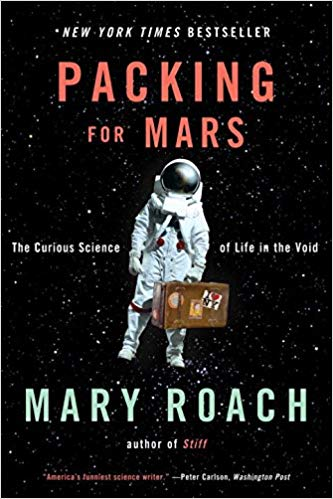
\includegraphics[width=\linewidth]{images/packing_for_mars.jpg}
   \varcaption{\href{https://wwnorton.com/books/9780393339918}{Publisher Link}, \href{https://www.amazon.com/Packing-Mars-Curious-Science-Life/dp/0393339912/}{Amazon Link}}
\end{marginfigure}

\begin{itemize}
    \item[] \textbf{Author:} Mary Roach
    \item[] \textbf{Published Year:} 2011
    \item[] \textbf{Publisher:} W. W. Norton \& Company
    \item[] \textbf{Number of Pages:} 336     
    \item[] \textbf{ISBN:} 9780393339918
    \item[] \textbf{Description:} The best-selling author of \textit{Stiff} and \textit{Bonk} explores the irresistibly strange universe of space travel and life without gravity. From the Space Shuttle training toilet to a crash test of NASA’s new space capsule, Mary Roach takes us on the surreally entertaining trip into the science of life in space and space on Earth.
\end{itemize}

\section*{A Short History of Nearly Everything: Special Illustrated Edition}

\begin{itemize}
    \item[] \textbf{Author:} Bill Bryson
    \item[] \textbf{Published Year:} 2010
    \item[] \textbf{Publisher:} Penguin Random House/Broadway
    \item[] \textbf{Number of Pages:} 624     
    \item[] \textbf{ISBN:} 9780307885159
    \item[] \textbf{Description:} The best-selling author of \textit{Stiff} and \textit{Bonk} explores the irresistibly strange universe of space travel and life without gravity. From the Space Shuttle training toilet to a crash test of NASA’s new space capsule, Mary Roach takes us on the surreally entertaining trip into the science of life in space and space on Earth.
\end{itemize}

\begin{marginfigure}[-10\baselineskip]
   
\includegraphics[width=\linewidth]{images/short_history_of_nearly_everything.jpg}
   \varcaption{\href{https://www.penguinrandomhouse.com/books/20549/a-short-history-of-nearly-everything-special-illustrated-edition-by-bill-bryson/}{Publisher Link}, \href{https://www.amazon.com/Short-History-Nearly-Everything-Illustrated/dp/0307885151/}{Amazon Link}}
\end{marginfigure}

\section*{Fermat's Enigma: The Epic Quest to Solve the World's \newline Greatest Mathematical Problem}
\begin{marginfigure}[\baselineskip]
   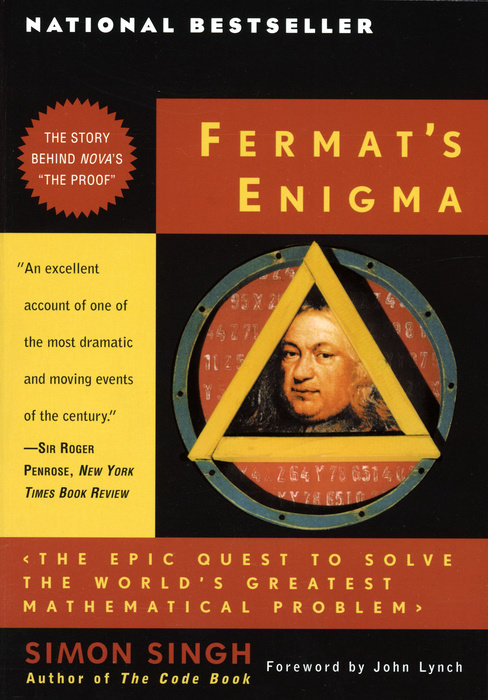
\includegraphics[width=\linewidth]{images/fermats_enigma.jpg}
   \varcaption{\href{https://www.penguinrandomhouse.com/books/168001/fermats-enigma-by-simon-singh-author-of-the-code-book-foreword-by-john-lynch/}{Publisher Link}, \href{https://www.amazon.com/Fermats-Enigma-Greatest-Mathematical-Problem/dp/0385493622/}{Amazon Link}}
\end{marginfigure}

\begin{itemize}
    \item[] \textbf{Author:} Simon Singh
    \item[] \textbf{Published Year:} 1998 
    \item[] \textbf{Publisher:} Penguin Random House/Anchor
    \item[] \textbf{Number of Pages:} 336      
    \item[] \textbf{ISBN:} 9780385493628
    \item[] \textbf{Description:} ``xn + yn = zn, where n represents 3, 4, 5, \ldots no solution. I have discovered a truly marvelous demonstration of this proposition which this margin is too narrow to contain.'' With these words, the seventeenth-century French mathematician Pierre de Fermat threw down the gauntlet to future generations. What came to be known as Fermat’s Last Theorem looked simple; proving it, however, became the Holy Grail of mathematics, baffling its finest minds for more than 350 years. In Fermat’s Enigma–based on the author’s award-winning documentary film, which aired on PBS’s "Nova"–Simon Singh tells the astonishingly entertaining story of the pursuit of that grail, and the lives that were devoted to, sacrificed for, and saved by it. Here is a mesmerizing tale of heartbreak and mastery that will forever change your feelings about mathematics.
\end{itemize}

\section*{Jam}
\begin{marginfigure}[\baselineskip]
   
\includegraphics[width=\linewidth]{images/jam.jpg}
   \varcaption{\href{https://www.darkhorse.com/Books/18-937/JAM-novel}{Publisher Link}, \href{https://www.amazon.com/Jam-Yahtzee-Croshaw/dp/1506706347/}{Amazon Link}}
\end{marginfigure}

\begin{itemize}
    \item[] \textbf{Author:} Yahtzee Croshaw
    \item[] \textbf{Published Year:} 2018
    \item[] \textbf{Publisher:} Dark Horse
    \item[] \textbf{Number of Pages:} 320      
    \item[] \textbf{ISBN:} 9781506706344
    \item[] \textbf{Description:} We were prepared for an earthquake. We had a flood plan in place. We could even have dealt with zombies. Probably. But no one expected the end to be quite so\ldots sticky\ldots or strawberry scented.
\end{itemize}

\section*{Earthsea, The First Four Books: A Wizard of Earthsea * The Tombs of Atuan * The Farthest Shore * Tehanu}
\begin{marginfigure}[12\baselineskip]
   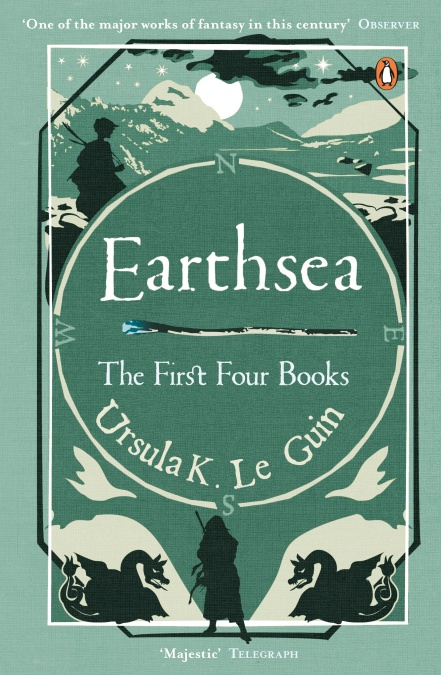
\includegraphics[width=\linewidth]{images/earthsea.jpg}
   \varcaption{\href{https://www.penguin.co.uk/books/149/14981/earthsea/9780241956878.html}{Publisher Link}, \href{https://www.amazon.com/Earthsea-Quartet-Ursula-Guin/dp/0241956870/}{Amazon Link}}
\end{marginfigure}

\begin{itemize}
    \item[] \textbf{Author:} Ursula K. Le Guin
    \item[] \textbf{Published Year:} 2012
    \item[] \textbf{Publisher:} Penguin Random House/Penguin
    \item[] \textbf{Number of Pages:} 704      
    \item[] \textbf{ISBN:} 9780241956878
    \item[] \textbf{Description:} Ged is but a goatherd on the island of Gont when he comes by his strange powers over nature. Sent to the School of Wizards on Roke, he learns the true way of magic and proves himself a powerful magician. And it is as the Archmage Sparrowhawk that he helps the High Priestess Tenar escape the labyrinth of darkness. But over the years, Ged witnesses true magic and the ancient ways submit to the forces of evil and death. Will he too succumb, or can he hold them back?
\end{itemize}

\section*{Machine Learning: The Art and Science of Algorithms that Make Sense of Data}
\begin{marginfigure}[3\baselineskip]
   
\includegraphics[width=\linewidth]{images/machine_learning.jpg}
   \varcaption{\href{https://www.cambridge.org/us/academic/subjects/computer-science/pattern-recognition-and-machine-learning/machine-learning-art-and-science-algorithms-make-sense-data?format=PB&isbn=9781107422223}{Publisher Link}, \href{https://www.amazon.com/Machine-Learning-Science-Algorithms-Sense/dp/1107422221/}{Amazon Link}}
\end{marginfigure}

\begin{itemize}
    \item[] \textbf{Author:} Peter Flach
    \item[] \textbf{Published Year:} 2012
    \item[] \textbf{Publisher:} Cambridge University
    \item[] \textbf{Number of Pages:} 409      
    \item[] \textbf{ISBN:} 9781107422223
    \item[] \textbf{Description:} As one of the most comprehensive machine learning texts around, this book does justice to the field's incredible richness, but without losing sight of the unifying principles. Peter Flach's clear, example-based approach begins by discussing how a spam filter works, which gives an immediate introduction to machine learning in action, with a minimum of technical fuss. Flach provides case studies of increasing complexity and variety with well-chosen examples and illustrations throughout. He covers a wide range of logical, geometric and statistical models and state-of-the-art topics such as matrix factorisation and ROC analysis. Particular attention is paid to the central role played by features. The use of established terminology is balanced with the introduction of new and useful concepts, and summaries of relevant background material are provided with pointers for revision if necessary. These features ensure Machine Learning will set a new standard as an introductory textbook.
\end{itemize}

\section*{This Book Is Full of Spiders: Seriously, Dude, Don't Touch It (John and Dave Book 2)}
\begin{marginfigure}[12\baselineskip]
   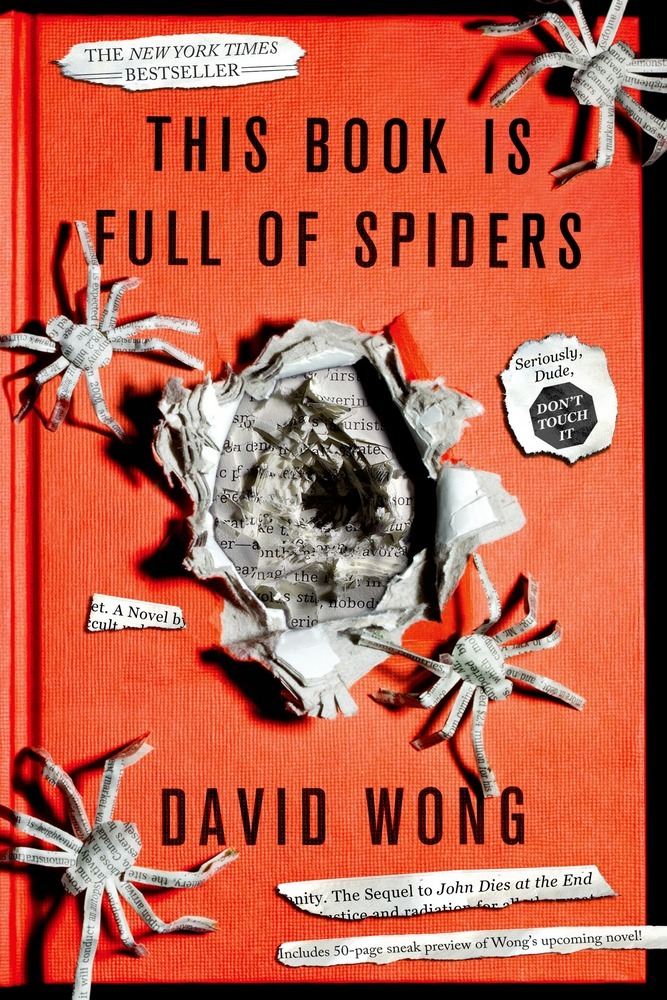
\includegraphics[width=\linewidth]{images/this_book_is_full_of_spiders.jpg}
   \varcaption{\href{https://us.macmillan.com/books/9781250036650}{Publisher Link}, \href{https://www.amazon.com/gp/product/1250036658/}{Amazon Link}}
\end{marginfigure}

\begin{itemize}
    \item[] \textbf{Author:} David Wong
    \item[] \textbf{Published Year:} 2013
    \item[] \textbf{Publisher:} Macmillan/St. Martin's Griffin
    \item[] \textbf{Number of Pages:} 464      
    \item[] \textbf{ISBN:} 9781250036650
    \item[] \textbf{Description:} Warning: You may have a huge, invisible spider living in your skull. THIS IS NOT A METAPHOR. You will dismiss this as ridiculous fear-mongering. Dismissing things as ridiculous fear-mongering is, in fact, the first symptom of parasitic spider infection --- the creature stimulates skepticism, in order to prevent you from seeking a cure. That's just as well, since the ``cure'' involves learning what a chainsaw tastes like. You can't feel the spider, because it controls your nerve endings. You won't even feel it when it breeds. And it will breed. Just stay calm, and remember that telling you about the spider situation is not the same as having caused it. I'm just the messenger. Even if I did sort of cause it. Either way, I won't hold it against you if you're upset. I know that's just the spider talking.
\end{itemize}

\section*{The Athenian Murders}
\begin{marginfigure}[10\baselineskip]
   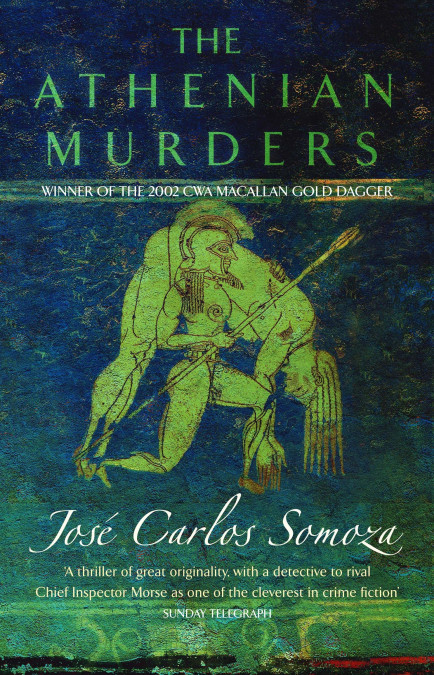
\includegraphics[width=\linewidth]{images/athenian_murders.jpg}
   \varcaption{\href{https://www.littlebrown.co.uk/titles/jose-carlos-somoza/the-athenian-murders/9780349116181/}{Publisher Link}, \href{https://www.amazon.com/Athenian-Murders-Jose-Carlos-Somoza/dp/0349116180/}{Amazon Link}}
\end{marginfigure}

\begin{itemize}
    \item[] \textbf{Author:} José Carlos Somoza
    \item[] \textbf{Published Year:} 2002
    \item[] \textbf{Publisher:} Little, Brown/Abacus
    \item[] \textbf{Number of Pages:} 320      
    \item[] \textbf{ISBN:} 9780349116181
    \item[] \textbf{Description:} \textit{The Athenian Murders} is a brilliant, very entertaining and absolutely original literary mystery, revolving round two intertwined riddles. In classical Athens, one of the pupils of Plato’s Academy is found dead. His idealistic teacher suspects that this wasn’t an accident and asks Herakles, known as the ‘Decipherer of Enigmas’, to investigate the death and ultimately a dark, irrational and subversive cult. The second plot unfolds in parallel through the footnotes of the translator of the text. As he proceeds with his work, he becomes increasingly convinced that the original author has hidden a second meaning, which can be brought to light by interpreting certain repeated words and images. As the main plot and also the translation of the manuscript advances, there are certain sinister coincidences, and it seems that the text is addressing him personally and in an increasingly menacing manner\ldots \end{itemize}

\section*{The Crying of Lot 49}
\begin{marginfigure}[17\baselineskip]
   
\includegraphics[width=\linewidth]{images/crying_of_lot_49.jpg}
   \varcaption{\href{https://www.harpercollins.com/9780062334411/the-crying-of-lot-49/}{Publisher Link}, \href{https://www.amazon.com/Crying-Lot-Perennial-Fiction-Library/dp/006091307X}{Amazon Link}}
\end{marginfigure}

\begin{itemize}
    \item[] \textbf{Author:} Thomas Pynchon
    \item[] \textbf{Published Year:} 2014
    \item[] \textbf{Publisher:} Harper Collins/Harper Perennial
    \item[] \textbf{Number of Pages:} 160      
    \item[] \textbf{ISBN:} 9780062334411
    \item[] \textbf{Description:} When her ex-lover, wealthy real-estate tycoon Pierce Inverarity dies and designates her the co-executor of his estate, California housewife Oedipa Mass is thrust into a paranoid mystery of metaphors, symbols, and the United States Postal Service. Traveling across Southern California, she meets some extremely interesting characters, and attains a not-inconsiderable amount of self-knowledge.
\end{itemize}

\section*{Snow Crash}
\begin{marginfigure}[\baselineskip]
   
\includegraphics[width=\linewidth]{images/snow_crash.jpg}
   \varcaption{\href{https://www.penguinrandomhouse.com/books/172832/snow-crash-by-neal-stephenson/}{Publisher Link}, \href{https://www.amazon.com/Snow-Crash-Neal-Stephenson/dp/0553380958}{Amazon Link}}
\end{marginfigure}

\begin{itemize}
    \item[] \textbf{Author:} Neal Stephenson
    \item[] \textbf{Published Year:} 2000
    \item[] \textbf{Publisher:} Penguin Random House/Del Rey
    \item[] \textbf{Number of Pages:} 440      
    \item[] \textbf{ISBN:} 9780553380958
    \item[] \textbf{Description:} In reality, Hiro Protagonist delivers pizza for Uncle Enzo’s CosoNostra Pizza Inc., but in the Metaverse he’s a warrior prince. Plunging headlong into the enigma of a new computer virus that’s striking down hackers everywhere, he races along the neon-lit streets on a search-and-destroy mission for the shadowy virtual villain threatening to bring about infocalypse.
\end{itemize}

\section*{The Silk Roads: A New History of the World}
\begin{marginfigure}[12\baselineskip]
   
\includegraphics[width=\linewidth]{images/silk_roads.jpg}
   \varcaption{\href{https://www.penguinrandomhouse.com/books/253699/the-silk-roads-by-peter-frankopan/9781101912379/}{Publisher Link}, \href{https://www.amazon.com/Silk-Roads-New-History-World/dp/1101912375/}{Amazon Link}}
\end{marginfigure}

\begin{itemize}
    \item[] \textbf{Author:} Peter Frankopan
    \item[] \textbf{Published Year:} 2017
    \item[] \textbf{Publisher:} Penguin Random House/Vintage
    \item[] \textbf{Number of Pages:} 672      
    \item[] \textbf{ISBN:} 9781101912379
    \item[] \textbf{Description:} Far more than a history of the Silk Roads, this book is truly a revelatory new history of the world, promising to destabilize notions of where we come from and where we are headed next. From the Middle East and its political instability to China and its economic rise, the vast region stretching eastward from the Balkans across the steppe and South Asia has been thrust into the global spotlight in recent years. Frankopan teaches us that to understand what is at stake for the cities and nations built on these intricate trade routes, we must first understand their astounding pasts. Frankopan realigns our understanding of the world, pointing us eastward. It was on the Silk Roads that East and West first encountered each other through trade and conquest, leading to the spread of ideas, cultures and religions. From the rise and fall of empires to the spread of Buddhism and the advent of Christianity and Islam, right up to the great wars of the twentieth century --- this book shows how the fate of the West has always been inextricably linked to the East.
\end{itemize}

\section*{The Righteous Mind: Why Good People Are Divided by Politics and Religion}

\begin{itemize}
    \item[] \textbf{Author:} Jonathan Haidt
    \item[] \textbf{Published Year:} 2013
    \item[] \textbf{Publisher:} Penguin Random House/Vintage
    \item[] \textbf{Number of Pages:} 528      
    \item[] \textbf{ISBN:} 9780307455772
    \item[] \textbf{Description:} Drawing on his twenty five years of groundbreaking research on moral psychology, Haidt shows how moral judgments arise not from reason but from gut feelings. He shows why liberals, conservatives, and libertarians have such different intuitions about right and wrong, and he shows why each side is actually right about many of its central concerns. In this subtle yet accessible book, Haidt gives you the key to understanding the miracle of human cooperation, as well as the curse of our eternal divisions and conflicts. If you’re ready to trade in anger for understanding, read \textit{The Righteous Mind}.
\end{itemize}

\begin{marginfigure}[-16\baselineskip]
   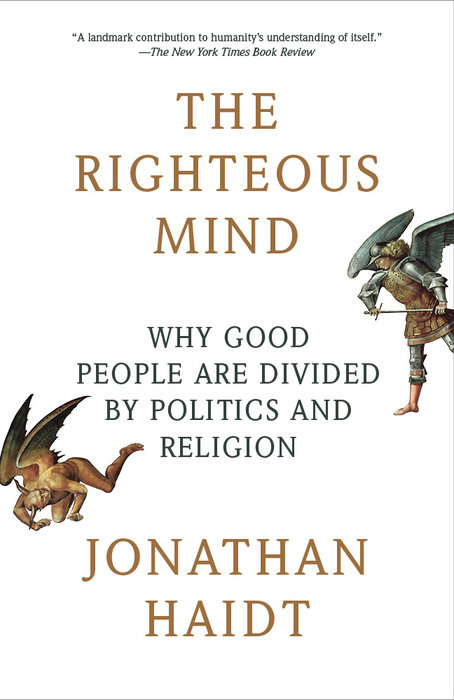
\includegraphics[width=\linewidth]{images/righteous_mind.jpg}
   \varcaption{\href{https://www.penguinrandomhouse.com/books/73535/the-righteous-mind-by-jonathan-haidt/}{Publisher Link}, \href{https://www.amazon.com/Righteous-Mind-Divided-Politics-Religion/dp/0307455777}{Amazon Link}}
\end{marginfigure}

\section*{Re: Colonised Planet 5, Shikasta (Canopus in Argos: \newline Archives Book 1)}
\begin{marginfigure}[\baselineskip]
   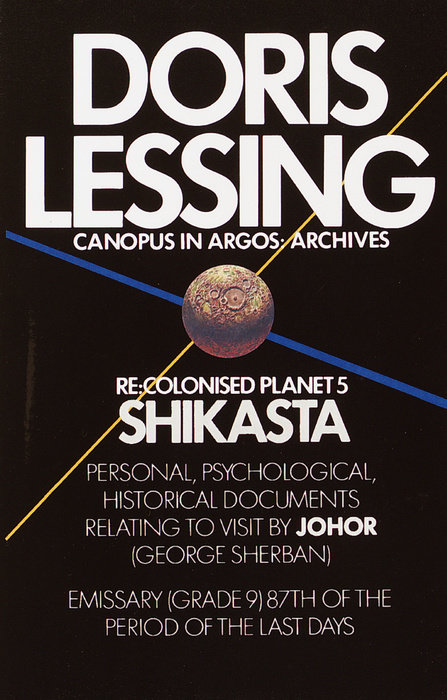
\includegraphics[width=\linewidth]{images/shikasta.jpg}
   \varcaption{\href{https://www.penguinrandomhouse.com/books/100291/shikasta-by-doris-lessing/9780394749778/}{Publisher Link}, \href{https://www.amazon.com/Shikasta-Colonised-Planet-Vintage-International/dp/0394749774/}{Amazon Link}}
\end{marginfigure}

\begin{itemize}
    \item[] \textbf{Author:} Donna Lessing
    \item[] \textbf{Published Year:} 1981
    \item[] \textbf{Publisher:} Penguin Random House/Vintage
    \item[] \textbf{Number of Pages:} 384      
    \item[] \textbf{ISBN:} 9780394749778
    \item[] \textbf{Description:} This is the first volume in the series of novels Doris Lessing calls collectively \textit{Canopus in Argos: Archives.} Presented as a compilation of documents, reports, letters, speeches and journal entries, this purports to be a general study of the planet Shikasta --- clearly the planet Earth --- to be used by history students of the higher planet Canopus and to be stored in the Canopian archives. For eons, galactic empires have struggled against one another, and Shikasta is one of the main battlegrounds. Johar, an emissary from Canopus and the primary contributor to the archives, visits Shikasta over the millennia from the time of the giants and the biblical great flood up to the present. With every visit he tries to distract Shikastans from the evil influences of the planet Shammat but notes with dismay the ever-growing chaos and destruction of Shikasta as its people hurl themselves towards World War III and annihilation.
\end{itemize}

\section*{Bad Days in History: A Gleefully Grim Chronicle of Misfortune, Mayhem, and Misery for Every Day of the Year}
\begin{marginfigure}[8\baselineskip]
   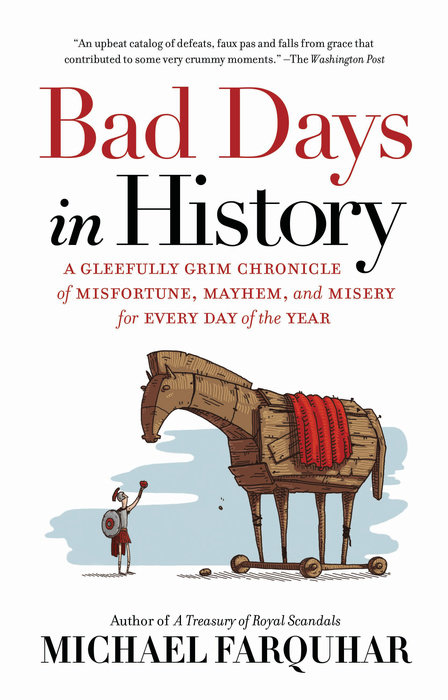
\includegraphics[width=\linewidth]{images/bad_days_in_history.jpg}
   \varcaption{\href{https://www.penguinrandomhouse.com/books/232075/bad-days-in-history-by-michael-farquhar/}{Publisher Link}, \href{https://www.amazon.com/Bad-Days-History-Gleefully-Misfortune/dp/1426218079/}{Amazon Link}}
\end{marginfigure}

\begin{itemize}
    \item[] \textbf{Author:} Michael Farquhar
    \item[] \textbf{Published Year:} 2017
    \item[] \textbf{Publisher:} Penguin Random House/National Geographic
    \item[] \textbf{Number of Pages:} 480      
    \item[] \textbf{ISBN:} 9781426218071
    \item[] \textbf{Description:} National Geographic author Michael Farquhar uncover an instance of bad luck, epic misfortune, and unadulterated mayhem tied to every day of the year. From Caligula’s blood-soaked end to hotelier Steve Wynn’s unfortunate run-in with a priceless Picasso, these 365 tales of misery include lost fortunes (like the would-be Apple investor who pulled out in 1977 and missed out on a \$30 billion-dollar windfall), romance gone wrong (like the 16th-century Shah who experimented with an early form of Viagra with empire-changing results), and truly bizarre moments (like the Great Molasses Flood of 1919). Think you’re having a bad day? Trust us, it gets worse.
\end{itemize}

\section*{Raft (Xeelee Sequence Book 1)}
\begin{marginfigure}[19\baselineskip]
   \includegraphics[width=\linewidth]{images/raft.jpg}
   \varcaption{\href{https://www.sfgateway.com/titles/stephen-baxter/raft/9780575127975/}{Publisher Link}, \href{https://www.amazon.com/Raft-Stephen-Baxter-author/dp/1473224055/}{Amazon Link}}
\end{marginfigure}

\begin{itemize}
    \item[] \textbf{Author:} Stephen Baxter
    \item[] \textbf{Published Year:} 2013
    \item[] \textbf{Publisher:} Orion/Gateway
    \item[] \textbf{Number of Pages:} 264      
    \item[] \textbf{ISBN:} 9781473224056
    \item[] \textbf{Description:} A spaceship from Earth accidentally crossed through a hole in space-time to a universe where the force of gravity is one billion times as strong as the gravity we know. Somehow the crew survived, aided by the fact that they emerged into a cloud of gas surrounding a black hole, which provided a breathable atmosphere. Five hundred years later, their descendants still struggle for existence, divided into two main groups. The Miners live on the Belt, a ramshackle ring of dwellings orbiting the core of a dead star, which they excavate for raw materials. These can be traded for food from the Raft, a structure built from the wreckage of the ship, on which a small group of scientists preserve the ancient knowledge which makes survival possible. Rees is a Miner whose curiosity about his world makes him stow away on a flying tree --- just one of the many strange local lifeforms --- carrying trade between the Belt and the Raft. And what he finds will change his world\ldots \end{itemize}

\section*{Good Omens: The Nice and Accurate Prophecies of Agnes Nutter, Witch}
\begin{marginfigure}[9\baselineskip]
   \includegraphics[width=\linewidth]{images/good_omens.jpg}
   \varcaption{\href{https://www.harpercollins.com/9780060853983/good-omens/}{Publisher Link}, \href{https://www.amazon.com/Good-Omens-Accurate-Prophecies-Nutter/dp/0060853980}{Amazon Link}}
\end{marginfigure}

\begin{itemize}
    \item[] \textbf{Author:} Neil Gaiman, Terry Pratchett
    \item[] \textbf{Published Year:} 2006
    \item[] \textbf{Publisher:} Harper Collins/William Morrow
    \item[] \textbf{Number of Pages:} 512      
    \item[] \textbf{ISBN:} 9780060853983
    \item[] \textbf{Description:} According to The Nice and Accurate Prophecies of Agnes Nutter, Witch (the world's only completely accurate book of prophecies, written in 1655, before she exploded), the world will end on a Saturday. Next Saturday, in fact. Just before dinner. So the armies of Good and Evil are amassing, Atlantis is rising, frogs are falling, tempers are flaring. Everything appears to be going according to Divine Plan. Except a somewhat fussy angel and a fast-living demon --- both of whom have lived amongst Earth's mortals since \emph{The Beginning} and have grown rather fond of the lifestyle --- are not actually looking forward to the coming Rapture. And someone seems to have misplaced the Antichrist\ldots \end{itemize}

\section*{Will Save the Galaxy for Food}
\begin{marginfigure}[7\baselineskip]
   \includegraphics[width=\linewidth]{images/will_save_galaxy_for_food.jpg}
   \varcaption{\href{https://www.darkhorse.com/Books/30-574/Will-Save-the-Galaxy-for-Food-TPB}{Publisher Link}, \href{https://www.amazon.com/Will-Save-Galaxy-Yahtzee-Croshaw/dp/1506701655/}{Amazon Link}}
\end{marginfigure}

\begin{itemize}
    \item[] \textbf{Author:} Yahtzee Croshaw
    \item[] \textbf{Published Year:} 2017
    \item[] \textbf{Publisher:} Dark Horse
    \item[] \textbf{Number of Pages:} 288      
    \item[] \textbf{ISBN:} 9781506701653
    \item[] \textbf{Description:} A not-quite-epic science-fiction adventure about a down-on-his-luck galactic pilot caught in a cross-galaxy struggle for survival! Space travel just isn’t what it used to be. With the invention of quantum teleportation, space heroes aren’t needed anymore. When one unlucky ex-adventurer masquerades as a famous pilot who is also a hated public figure, he’s sucked into ever-deepening corporate and political intrigue. Between space pirates, adorable but deadly creatures, and a missing fortune in royalties, saving the universe was never this difficult!
\end{itemize}

\section*{Consider Phlebas (Culture Series Book 1)}
\begin{marginfigure}[8\baselineskip]
   \includegraphics[width=\linewidth]{images/consider_phlebas.jpg}
   \varcaption{\href{https://www.hachettebookgroup.com/titles/iain-m-banks/consider-phlebas/9780316095839/}{Publisher Link}, \href{https://www.amazon.com/Consider-Phlebas-Culture-Iain-Banks/dp/031600538X/}{Amazon Link}}
\end{marginfigure}

\begin{itemize}
    \item[] \textbf{Author:} Iain M. Banks
    \item[] \textbf{Published Year:} 2008
    \item[] \textbf{Publisher:} Hachette/Orbit
    \item[] \textbf{Number of Pages:} 544      
    \item[] \textbf{ISBN:} 9780316095839
    \item[] \textbf{Description:} The war raged across the galaxy. Billions had died, billions more were doomed. Moons, planets, the very stars themselves, faced destruction, cold-blooded, brutal, and worse, random. The Idirans fought for their Faith; the Culture for its moral right to exist. Principles were at stake. There could be no surrender. Within the cosmic conflict, an individual crusade. Deep within a fabled labyrinth on a barren world, a Planet of the Dead proscribed to mortals, lay a fugitive Mind. Both the Culture and the Idirans sought it. It was the fate of Horza, the Changer, and his motley crew of unpredictable mercenaries, human and machine, actually to find it, and with it their own destruction.
\end{itemize}

\section*{The Silmarillion}
\begin{marginfigure}[6\baselineskip]
   \includegraphics[width=\linewidth]{images/silmarillion.jpg}
   \varcaption{\href{http://www.harpercollins.co.uk/9780007523221/the-silmarillion/}{Publisher Link}, \href{https://www.amazon.com/Silmarillion-J-R-R-Tolkien/dp/0544338014}{Amazon Link}}
\end{marginfigure}

\begin{itemize}
    \item[] \textbf{Author:} J. R. R. Tolkien
    \item[] \textbf{Published Year:} 2014
    \item[] \textbf{Publisher:} Harper Collins/Mariner
    \item[] \textbf{Number of Pages:} 384      
    \item[] \textbf{ISBN:} 9780007523221
    \item[] \textbf{Description:} The Silmarillion is an account of the Elder Days, of the First Age of Tolkien’s world. It is the ancient drama to which the characters in The Lord of the Rings look back, and in whose events some of them such as Elrond and Galadriel took part. The tales of The Silmarillion are set in an age when Morgoth, the first Dark Lord, dwelt in Middle-Earth, and the High Elves made war upon him for the recovery of the Silmarils, the jewels containing the pure light of Valinor. Included in the book are several shorter works. The Ainulindale is a myth of the Creation and in the Valaquenta the nature and powers of each of the gods is described. The Akallabeth recounts the downfall of the great island kingdom of Númenor at the end of the Second Age and Of the Rings of Power tells of the great events at the end of the Third Age, as narrated in The Lord of the Rings.
\end{itemize}

\section*{Hyperion (Hyperion Cantos Book 1)}
\begin{marginfigure}[11\baselineskip]
   \includegraphics[width=\linewidth]{images/hyperion.jpg}
   \varcaption{\href{https://www.penguinrandomhouse.com/books/167468/hyperion-by-dan-simmons/}{Publisher Link}, \href{https://www.amazon.com/Silmarillion-J-R-R-Tolkien/dp/0544338014}{Amazon Link}}
\end{marginfigure}

\begin{itemize}
    \item[] \textbf{Author:} Dan Simmons
    \item[] \textbf{Published Year:} 2017
    \item[] \textbf{Publisher:} Penguin Random House/Del Rey
    \item[] \textbf{Number of Pages:} 496      
    \item[] \textbf{ISBN:} 9780399178610
    \item[] \textbf{Description:} On the world called Hyperion, beyond the reach of galactic law, waits a creature called the Shrike. There are those who worship it. There are those who fear it. And there are those who have vowed to destroy it. In the Valley of the Time Tombs, where huge, brooding structures move backward through time, the Shrike waits for them all. On the eve of Armageddon, with the entire galaxy at war, seven pilgrims set forth on a final voyage to Hyperion seeking the answers to the unsolved riddles of their lives. Each carries a desperate hope --- and a terrible secret. And one may hold the fate of humanity in his hands.
\end{itemize}

\section*{What the Hell Did I Just Read: A Novel of Cosmic Horror (John and Dave Book 3)}
\begin{marginfigure}[5\baselineskip]
   \includegraphics[width=\linewidth]{images/what_the_hell_did_i_just_read.jpg}
   \varcaption{\href{https://us.macmillan.com/books/9781250040206}{Publisher Link}, \href{https://www.amazon.com/What-Hell-Did-Just-Read/dp/1250135311/}{Amazon Link}}
\end{marginfigure}

\begin{itemize}
    \item[] \textbf{Author:} David Wong
    \item[] \textbf{Published Year:} 2018
    \item[] \textbf{Publisher:} Macmillan/St. Martin's Griffin
    \item[] \textbf{Number of Pages:} 384      
    \item[] \textbf{ISBN:} 9781250135315
    \item[] \textbf{Description:} It's the story ``They'' don't want you to read. Though, to be fair, ``They'' are probably right about this one. To quote the Bible, ``Learning the truth can be like loosening a necktie, only to realize it was the only thing keeping your head attached.'' No, don't put the book back on the shelf --- it is now your duty to purchase it to prevent others from reading it. Yes, it works with e-books, too, I don't have time to explain how. While investigating a fairly straightforward case of a shape-shifting interdimensional child predator, Dave, John and Amy realized there might actually be something weird going on. Together, they navigate a diabolically convoluted maze of illusions, lies, and their own incompetence in an attempt to uncover a terrible truth they --- like you --- would be better off not knowing. Your first impulse will be to think that a story this gruesome --- and, to be frank, stupid --- cannot possibly be true. That is precisely the reaction ``They'' are hoping for.
\end{itemize}

\section*{Do Androids Dream of Electric Sheep?}

\begin{marginfigure}[17\baselineskip]
   \includegraphics[width=\linewidth]{images/do_androids_dream_of_electric_sheep.jpg}
   \varcaption{\href{https://www.penguinrandomhouse.com/books/40617/do-androids-dream-of-electric-sheep-by-philip-k-dick/}{Publisher Link}, \href{https://www.amazon.com/Androids-Dream-Electric-Sheep-inspiration/dp/0345404475}{Amazon Link}}
\end{marginfigure}

\begin{itemize}
    \item[] \textbf{Author:} Philip K. Dick
    \item[] \textbf{Published Year:} 1996
    \item[] \textbf{Publisher:} Penguin Random House/Del Rey
    \item[] \textbf{Number of Pages:} 240      
    \item[] \textbf{ISBN:} 9780345404473
    \item[] \textbf{Description:} By 2021, the World War has killed millions, driving entire species into extinction and sending mankind off-planet. Those who remain covet any living creature, and for people who can’t afford one, companies built incredibly realistic simulacra: horses, birds, cats, sheep. They’ve even built humans. Immigrants to Mars receive androids so sophisticated they are indistinguishable from true men or women. Fearful of the havoc these artificial humans can wreak, the government bans them from Earth. Driven into hiding, unauthorized androids live among human beings, undetected. Rick Deckard, an officially sanctioned bounty hunter, is commissioned to find rogue androids and ``retire'' them. But when cornered, androids fight back --- with lethal force.
\end{itemize}

\section*{Embassytown}
\begin{marginfigure}[9\baselineskip]
   \includegraphics[width=\linewidth]{images/embassytown.jpg}
   \varcaption{\href{https://www.penguinrandomhouse.com/books/206876/embassytown-by-china-mieville/9780345524508/}{Publisher Link}, \href{https://www.amazon.com/Embassytown-Novel-China-Miéville/dp/0345524500/}{Amazon Link}}
\end{marginfigure}

\begin{itemize}
    \item[] \textbf{Author:} China Miéville
    \item[] \textbf{Published Year:} 2012
    \item[] \textbf{Publisher:} Penguin Random House/Del Rey
    \item[] \textbf{Number of Pages:} 368      
    \item[] \textbf{ISBN:} 9780345524508
    \item[] \textbf{Description:} In the far future, humans have colonized a distant planet, home to the enigmatic Ariekei, sentient beings famed for a language unique in the universe, one that only a few altered human ambassadors can speak. Avice Benner Cho, a human colonist, has returned to Embassytown after years of deep-space adventure. She cannot speak the Ariekei tongue, but she is an indelible part of it, having long ago been made a figure of speech, a living simile in their language. When distant political machinations deliver a new ambassador to Arieka, the fragile equilibrium between humans and aliens is violently upset. Catastrophe looms, and Avice is torn between competing loyalties: to a husband she no longer loves, to a system she no longer trusts, and to her place in a language she cannot speak --- but which speaks through her, whether she likes it or not.

\end{itemize}

\section*{The Illuminatus! Trilogy: The Eye in the Pyramid, The Golden \newline Apple, Leviathan}

\begin{itemize}
    \item[] \textbf{Author:} Robert Shea \& Robert Anton Wilson
    \item[] \textbf{Published Year:} 1983
    \item[] \textbf{Publisher:} Penguin Random House/Dell
    \item[] \textbf{Number of Pages:} 816      
    \item[] \textbf{ISBN:} 9780440539810
    \item[] \textbf{Description:} It was a deadly mistake. Joseph Malik, editor of a radical magazine, had snooped into rumors about an ancient secret society that was still alive and kicking. Now his offices have been bombed, he's missing, and the case has landed in the lap of a tough, cynical, streetwise New York detective. Saul Goodman knows he's stumbled onto something big --- but even he can't guess how far into the pinnacles of power this conspiracy of evil has penetrated. Filled with sex and violence --- in and out of time and space --- the three books of \textit{The Illuminatus! Trilogy} are only partly works of the imagination. They tackle all the cover-ups of our time --- from who really shot the Kennedys to why there's a pyramid on a one-dollar bill --- and suggest a mind-blowing truth.
\end{itemize}

\begin{marginfigure}[-43\baselineskip]
   \includegraphics[width=\linewidth]{images/illuminatus.jpg}
   \varcaption{\href{https://www.penguinrandomhouse.com/books/165363/the-illuminatus-trilogy-by-robert-shea-and-robert-anton-wilson/}{Publisher Link}, \href{https://www.amazon.com/Illuminatus-Trilogy-Pyramid-Golden-Leviathan/dp/0440539811}{Amazon Link}}
\end{marginfigure}

\section*{American Gods}

\begin{itemize}
    \item[] \textbf{Author:} Neil Gaiman
    \item[] \textbf{Published Year:} 2013
    \item[] \textbf{Publisher:} Harper Collins/William Morrow
    \item[] \textbf{Number of Pages:} 560      
    \item[] \textbf{ISBN:} 9780062080233
    \item[] \textbf{Description:} Locked behind bars for three years, Shadow did his time, quietly waiting for the day when he could return to Eagle Point, Indiana. A man no longer scared of what tomorrow might bring, all he wanted was to be with Laura, the wife he deeply loved, and start a new life. But just days before his release, Laura and Shadow’s best friend are killed in an accident. With his life in pieces and nothing to keep him tethered, Shadow accepts a job from a beguiling stranger he meets on the way home, an enigmatic man who calls himself Mr. Wednesday. A trickster and a rogue, Wednesday seems to know more about Shadow than Shadow does himself. Life as Wednesday’s bodyguard, driver, and errand boy is far more interesting and dangerous than Shadow ever imagined. Soon Shadow learns that the past never dies\ldots and that beneath the placid surface of everyday life a storm is brewing --- an epic war for the very soul of America --- and that he is standing squarely in its path.
\end{itemize}

\begin{marginfigure}[-36\baselineskip]
   \includegraphics[width=\linewidth]{images/american_gods.jpg}
   \varcaption{\href{https://www.harpercollins.com/9780062080233/american-gods/}{Publisher Link}, \href{https://www.amazon.com/American-Gods-Novel-Neil-Gaiman/dp/0062572237/}{Amazon Link}}
\end{marginfigure}

\section*{Player of Games (Culture Series Book 2)}
\begin{marginfigure}[1\baselineskip]
   \includegraphics[width=\linewidth]{images/player_of_games.jpg}
   \varcaption{\href{https://www.hachettebookgroup.com/titles/iain-m-banks/the-player-of-games/9780316005401/}{Publisher Link}, \href{https://www.amazon.com/Player-Games-Culture-Iain-Banks/dp/0316005401/}{Amazon Link}}
\end{marginfigure}

\begin{itemize}
    \item[] \textbf{Author:} Iain M. Banks
    \item[] \textbf{Published Year:} 2008
    \item[] \textbf{Publisher:} Hachette/Orbit
    \item[] \textbf{Number of Pages:} 416      
    \item[] \textbf{ISBN:} 9780316005401
    \item[] \textbf{Description:} The Culture --- a human/machine symbiotic society – has thrown up many great Game Players, and one of the greatest is Gurgeh. Jernau Morat Gurgeh. The Player of Games. Master of every board, computer and strategy. Bored with success, Gurgeh travels to the Empire of Azad, cruel and incredibly wealthy, to try their fabulous game\ldots a game so complex, so like life itself, that the winner becomes emperor. Mocked, blackmailed, almost murdered, Gurgeh accepts the game, and with it the challenge of his life --- and very possibly his death.

\end{itemize}

\section*{Borne}
\begin{marginfigure}[5\baselineskip]
   \includegraphics[width=\linewidth]{images/borne.jpg}
   \varcaption{\href{https://us.macmillan.com/books/9780374115241}{Publisher Link}, \href{https://www.amazon.com/Borne-Novel-Jeff-VanderMeer/dp/0374537658/}{Amazon Link}}
\end{marginfigure}

\begin{itemize}
    \item[] \textbf{Author:} Jeff VanderMeer
    \item[] \textbf{Published Year:} 2017
    \item[] \textbf{Publisher:} Macmillan/MCD Farrar, Straus and Giroux
    \item[] \textbf{Number of Pages:} 336      
    \item[] \textbf{ISBN:} 9780374115241
    \item[] \textbf{Description:} In \textit{Borne}, a young woman named Rachel survives as a scavenger in a ruined city half destroyed by drought and conflict. The city is dangerous, littered with discarded experiments from the Company --- a biotech firm now derelict --- and punished by the unpredictable predations of a giant bear. Rachel ekes out an existence in the shelter of a run-down sanctuary she shares with her partner, Wick, who deals his own homegrown psychoactive biotech. One day, Rachel finds Borne during a scavenging mission and takes him home. Borne as salvage is little more than a green lump --- plant or animal? --- but exudes a strange charisma. Borne reminds Rachel of the marine life from the island nation of her birth, now lost to rising seas. There is an attachment she resents: in this world any weakness can kill you. Yet, against her instincts --- and definitely against Wick’s wishes --- Rachel keeps Borne. She cannot help herself. Borne, learning to speak, learning about the world, is fun to be with, and in a world so broken that innocence is a precious thing. For Borne makes Rachel see beauty in the desolation around her. She begins to feel a protectiveness she can ill afford. ``He was born, but I had borne him.'' But as Borne grows, he begins to threaten the balance of power in the city and to put the security of her sanctuary with Wick at risk. For the Company, it seems, may not be truly dead, and new enemies are creeping in. What Borne will lay bare to Rachel as he changes is how precarious her existence has been, and how dependent on subterfuge and secrets. In the aftermath, nothing may ever be the same.

\end{itemize}

\section*{The Marriages Between Zones Three, Four and Five (Canopus in Argos: Archives Book 2)}
\begin{marginfigure}[15\baselineskip]
   \includegraphics[width=\linewidth]{images/marriages_between_zones_three.jpg}
   \varcaption{\href{https://www.harpercollins.co.uk/9780007404223/the-marriages-between-zones-3-4-and-5-canopus-in-argos-archives-series-book-2/}{Publisher Link}, \href{https://www.amazon.com/Marriages-Between-Zones-Three-Four/dp/0006547206/}{Amazon Link}}
\end{marginfigure}

\begin{itemize}
    \item[] \textbf{Author:} Doris Lessing
    \item[] \textbf{Published Year:} 1994
    \item[] \textbf{Publisher:} Harper Collins
    \item[] \textbf{Number of Pages:} 304      
    \item[] \textbf{ISBN:} 9780006547204
    \item[] \textbf{Description:} This is the story of the kindly Queen of Zone Three, who rules a land free of all harshness, and her forced marriage with the soldier-king of Zone Four, which is hierarchic, disciplined, inflexible, dutiful. This apparently difficult marriage, unwanted by both, requires a compromise between impulse and reason, between instinct and logic. Ben Ata learns to accept and then to love the ruler of Zone Three and her alien ways; and she learns to love and to need him. But when the Queen is commanded by the Providers to return to her own realm, she must obey, shattering though it is to leave her husband and child. Ben Ata, in turn, is ordered to marry the savage beauty who rules Zone Five, a land that both unites and reverses the other two Zones.
\end{itemize}

\section*{Ubik}
\begin{marginfigure}[20\baselineskip]
   \includegraphics[width=\linewidth]{images/ubik.jpg}
   \varcaption{\href{https://www.hmhbooks.com/shop/books/Ubik/9780547572291}{Publisher Link}, \href{https://www.amazon.com/Ubik-Philip-K-Dick/dp/0547572298}{Amazon Link}}
\end{marginfigure}

\begin{itemize}
    \item[] \textbf{Author:} Philip K. Dick
    \item[] \textbf{Published Year:} 2012
    \item[] \textbf{Publisher:} Houghton Mifflin Harcourt/Mariner
    \item[] \textbf{Number of Pages:} 240      
    \item[] \textbf{ISBN:} 9780547572291
    \item[] \textbf{Description:} Glen Runciter runs a lucrative business --- deploying his teams of anti-psychics to corporate clients who want privacy and security from psychic spies. But when he and his top team are ambushed by a rival, he is gravely injured and placed in ``half-life'', a dreamlike state of suspended animation. Soon, though, the surviving members of the team begin experiencing some strange phenomena, such as Runciter’s face appearing on coins and the world seeming to move backward in time. As consumables deteriorate and technology gets ever more primitive, the group needs to find out what is causing the shifts and what a mysterious product called Ubik has to do with it all. 
\end{itemize}

\section*{Perdido Street Station (Bas-Lag Book 1)}

\begin{itemize}
    \item[] \textbf{Author:} China Miéville
    \item[] \textbf{Published Year:} 2001 
    \item[] \textbf{Publisher:} Penguin Random House/Del Rey
    \item[] \textbf{Number of Pages:} 720      
    \item[] \textbf{ISBN:} 9780345443021
    \item[] \textbf{Description:} Beneath the towering bleached ribs of a dead, ancient beast lies New Crobuzon, a squalid city where humans, Re-mades, and arcane races live in perpetual fear of Parliament and its brutal militia. The air and rivers are thick with factory pollutants and the strange effluents of alchemy, and the ghettos contain a vast mix of workers, artists, spies, junkies, and whores. In New Crobuzon, the unsavory deal is stranger to none—not even to Isaac, a brilliant scientist with a penchant for Crisis Theory. Isaac has spent a lifetime quietly carrying out his unique research. But when a half-bird, half-human creature known as the Garuda comes to him from afar, Isaac is faced with challenges he has never before fathomed. Though the Garuda’s request is scientifically daunting, Isaac is sparked by his own curiosity and an uncanny reverence for this curious stranger. While Isaac’s experiments for the Garuda turn into an obsession, one of his lab specimens demands attention: a brilliantly colored caterpillar that feeds on nothing but a hallucinatory drug and grows larger --- and more consuming --- by the day. What finally emerges from the silken cocoon will permeate every fiber of New Crobuzon—and not even the Ambassador of Hell will challenge the malignant terror it invokes\ldots \end{itemize}

\begin{marginfigure}[-44\baselineskip]
   \includegraphics[width=\linewidth]{images/perdido_street_station.jpg}
   \varcaption{\href{https://www.hmhbooks.com/shop/books/Ubik/9780547572291}{Publisher Link}, \href{https://www.amazon.com/Ubik-Philip-K-Dick/dp/0547572298}{Amazon Link}}
\end{marginfigure}

\section*{Solaris}
\begin{marginfigure}[1\baselineskip]
   \includegraphics[width=\linewidth]{images/solaris.jpg}
   \varcaption{\href{https://www.hmhbooks.com/shop/books/Solaris/9780156027601}{Publisher Link}, \href{https://www.amazon.com/Solaris-Stanislaw-Lem/dp/0156027607/}{Amazon Link}}
\end{marginfigure}

\begin{itemize}
    \item[] \textbf{Author:} Stanisław Lem
    \item[] \textbf{Published Year:} 2002 
    \item[] \textbf{Publisher:} Houghton Mifflin Harcourt/Mariner
    \item[] \textbf{Number of Pages:} 224      
    \item[] \textbf{ISBN:} 9780156027601
    \item[] \textbf{Description:} When psychologist Kris Kelvin arrives at the planet Solaris to study the ocean that covers its surface, he finds himself confronting a painful memory embodied in the physical likeness of a past lover. Kelvin learns that he is not alone in this and that other crews examining the planet are plagued with their own repressed and newly real memories. Could it be, as Solaris scientists speculate, that the ocean may be a massive neural center creating these memories, for a reason no one can identify?
\end{itemize}

\section*{Norse Mythology}
\begin{marginfigure}[2\baselineskip]
   \includegraphics[width=\linewidth]{images/norse_mythology.jpg}
   \varcaption{\href{https://wwnorton.com/books/9780393356182}{Publisher Link}, \href{https://www.amazon.com/Norse-Mythology-Neil-Gaiman/dp/0393356183/}{Amazon Link}}
\end{marginfigure}

\begin{itemize}
    \item[] \textbf{Author:} Neil Gaiman
    \item[] \textbf{Published Year:} 2018 
    \item[] \textbf{Publisher:} W. W. Norton \& Company
    \item[] \textbf{Number of Pages:} 304      
    \item[] \textbf{ISBN:} 9780393356182
    \item[] \textbf{Description:} In \textit{Norse Mythology}, Gaiman stays true to the myths in envisioning the major Norse pantheon: Odin, the highest of the high, wise, daring, and cunning; Thor, Odin’s son, incredibly strong yet not the wisest of gods; and Loki --- son of a giant --- blood brother to Odin and a trickster and unsurpassable manipulator. Gaiman fashions these primeval stories into a novelistic arc that begins with the genesis of the legendary nine worlds and delves into the exploits of deities, dwarfs, and giants. Through Gaiman’s deft and witty prose, these gods emerge with their fiercely competitive natures, their susceptibility to being duped and to duping others, and their tendency to let passion ignite their actions, making these long-ago myths breathe pungent life again.
\end{itemize}

\section*{Differently Morphous}
\begin{marginfigure}[9\baselineskip]
   \includegraphics[width=\linewidth]{images/differently_morphous.jpg}
   \varcaption{\href{https://www.darkhorse.com/Books/3003-029/Differently-Morphous-TPB}{Publisher Link}, \href{https://www.amazon.com/Differently-Morphous-Yahtzee-Croshaw/dp/1506711642/}{Amazon Link}}
\end{marginfigure}

\begin{itemize}
    \item[] \textbf{Author:} Yahtzee Croshaw
    \item[] \textbf{Published Year:} 2019 
    \item[] \textbf{Publisher:} Dark Horse
    \item[] \textbf{Number of Pages:} 304      
    \item[] \textbf{ISBN:} 9781506711645
    \item[] \textbf{Description:} A magical serial killer is on the loose, and gelatinous, otherworldly creatures are infesting the English countryside. Which is making life for the Ministry of Occultism difficult, because magic is supposed to be their best kept secret. After centuries in the shadows, the Ministry is forced to unmask, exposing the country's magical history --- and magical citizens --- to a brave new world of social media, government scrutiny, and public relations. On the trail of the killer are the Ministry's top agents: a junior operative with a photographic memory (and not much else), a couple of overgrown schoolboys with godlike powers, and a demonstrably insane magician. But as they struggle for results, their superiors at HQ must face the greatest threat the Ministry has ever known: the forces of political correctness\ldots \end{itemize}

\section*{Use of Weapons (Culture Series Book 3)}
\begin{marginfigure}[\baselineskip]
   \includegraphics[width=\linewidth]{images/use_of_weapons.jpg}
   \varcaption{\href{https://www.hachettebookgroup.com/titles/iain-m-banks/use-of-weapons/9780316030571/}{Publisher Link}, \href{https://www.amazon.com/Use-Weapons-Culture-Iain-Banks/dp/0316030570/}{Amazon Link}}
\end{marginfigure}

\begin{itemize}
    \item[] \textbf{Author:} Iain M. Banks
    \item[] \textbf{Published Year:} 2008 
    \item[] \textbf{Publisher:} Hachette/Orbit
    \item[] \textbf{Number of Pages:} 512      
    \item[] \textbf{ISBN:} 9780316030571
    \item[] \textbf{Description:} The man known as Cheradenine Zakalwe was one of Special Circumstances’ foremost agents, changing the destiny of planets to suit the Culture through intrigue, dirty tricks and military action. The woman known as Diziet Sma had plucked him from obscurity and pushed him towards his present eminence, but despite all their dealings she did not know him as well as she thought. The drone known as Skaffen-Amtiskaw knew both of these people. It had once saved the woman’s life by massacring her attackers in a particularly bloody manner. It believed the man to be a lost cause. But not even its machine could see the horrors in his past.
\end{itemize}

\section*{Going Bovine}
\begin{marginfigure}[13\baselineskip]
   \includegraphics[width=\linewidth]{images/going_bovine.jpg}
   \varcaption{\href{https://www.penguinrandomhouse.com/books/17786/going-bovine-by-libba-bray/9780385733984/}{Publisher Link}, \href{https://www.amazon.com/Going-Bovine-Libba-Bray/dp/0385733984}{Amazon Link}}
\end{marginfigure}

\begin{itemize}
    \item[] \textbf{Author:} Libba Bray
    \item[] \textbf{Published Year:} 2010 
    \item[] \textbf{Publisher:} Penguin Random House/Ember
    \item[] \textbf{Number of Pages:} 496      
    \item[] \textbf{ISBN:} 9780385733984
    \item[] \textbf{Description:} All 16-year-old Cameron wants is to get through high school --- and life in general --- with a minimum of effort. It’s not a lot to ask. But that’s before he’s given some bad news: he’s sick and he’s going to die. Which totally sucks. Hope arrives in the winged form of Dulcie, a loopy punk angel/possible hallucination with a bad sugar habit. She tells Cam there is a cure --- if he’s willing to go in search of it. With the help of a death-obsessed, video-gaming dwarf and a yard gnome, Cam sets off on the mother of all road trips through a twisted America\ldots into the heart of what matters most.
\end{itemize}

\section*{The Harper Collins Study Bible: Fully Revised \& Updated}
\begin{marginfigure}[5\baselineskip]
   \includegraphics[width=\linewidth]{images/bible.jpg}
   \varcaption{\href{https://www.harpercollins.com/9780061228407/the-harpercollins-study-bible/}{Publisher Link}, \href{https://www.amazon.com/HarperCollins-Study-Bible-Revised-Updated/dp/0061228400/}{Amazon Link}}
\end{marginfigure}

\begin{itemize}
    \item[] \textbf{Author:} Harold W. Attridge \& Society of Biblical Literature
    \item[] \textbf{Published Year:} 2006 
    \item[] \textbf{Publisher:} Harper Collins/HarperOne
    \item[] \textbf{Number of Pages:} 2272      
    \item[] \textbf{ISBN:} 9780061228407
    \item[] \textbf{Description:} The HarperCollins Study Bible is the landmark general reference Bible that offers the full text of the New Revised Standard Version as well as in-depth articles, introductions, and comprehensive notes by today's leading biblical scholars for the Society of Biblical Literature. Completely revised and updated, this edition incorporates the latest scholarship and findings as well as incorporating new diagrams, charts, and maps.
\end{itemize}

\section*{Cloud Atlas}
\begin{marginfigure}[18\baselineskip]
   \includegraphics[width=\linewidth]{images/cloud_atlas.jpg}
   \varcaption{\href{https://www.penguinrandomhouse.com/books/115430/cloud-atlas-by-david-mitchell/9780812994711/}{Publisher Link}, \href{https://www.amazon.com/Cloud-Atlas-Novel-David-Mitchell/dp/0375507256}{Amazon Link}}
\end{marginfigure}

\begin{itemize}
    \item[] \textbf{Author:} David Mitchell
    \item[] \textbf{Published Year:} 2004  
    \item[] \textbf{Publisher:} Penguin Random House/Random House
    \item[] \textbf{Number of Pages:} 528      
    \item[] \textbf{ISBN:} 9780375507250
    \item[] \textbf{Description:} Cloud Atlas begins in 1850 with Adam Ewing, an American notary voyaging from the Chatham Isles to his\ldots  Abruptly, the action jumps to Belgium in 1931, where Robert Frobisher, a disinherited bisexual composer, contrives his way into the household of an infirm maestro who has a beguiling wife and a nubile daughter\ldots From there we jump to the West Coast in the 1970s and a troubled reporter named Luisa Rey, who stumbles upon a web of corporate greed and murder that threatens to claim her life\ldots And onward, with dazzling virtuosity, to an inglorious present-day England; to a Korean superstate of the near future where neocapitalism has run amok; and, finally, to a postapocalyptic Iron Age Hawaii in the last days of history.
\end{itemize}

\section*{The Cost of Discipleship}

\begin{itemize}
    \item[] \textbf{Author:} Dietrich Bonhoeffer
    \item[] \textbf{Published Year:} 1995  
    \item[] \textbf{Publisher:} Simon \& Schuster/Touchstone
    \item[] \textbf{Number of Pages:} 320      
    \item[] \textbf{ISBN:} 9780684815008
    \item[] \textbf{Description:} What can the call to discipleship, the adherence to the word of Jesus, mean today to the businessman, the soldier, the laborer, or the government worker? What did Jesus mean to say to us? What is his will for us today? Drawing on the Sermon on the Mount, Dietrich Bonhoeffer answers these timeless questions by providing a seminal reading of the dichotomy between ``cheap grace'' and ``costly grace''. ``Cheap grace'', Bonhoeffer wrote, ``is the grace we bestow on ourselves\ldots grace without discipleship\ldots Costly grace is the gospel which must be sought again and again, the girl which must be asked for, the door at which a man must know\ldots It is costly because it costs a man his life, and it is grace because it gives a man the only true life.'' The Cost of Discipleship is a compelling statement of the demands of sacrifice and ethical consistency from a man whose life and thought were exemplary articulations of a new type of leadership inspired by the Gospel, and imbued with the spirit of Christian humanism and a creative sense of civic duty.
\end{itemize}

\begin{marginfigure}[-40\baselineskip]
   \includegraphics[width=\linewidth]{images/cost_of_discipleship.jpg}
   \varcaption{\href{https://www.simonandschuster.com/books/The-Cost-of-Discipleship/Dietrich-Bonhoeffer/9780684815008}{Publisher Link}, \href{https://www.amazon.com/gp/product/0684815001/}{Amazon Link}}
\end{marginfigure}

\section*{The Scar (Bas-Lag Book 2)}
\begin{marginfigure}[\baselineskip]
   \includegraphics[width=\linewidth]{images/scar.jpg}
   \varcaption{\href{https://www.penguinrandomhouse.com/books/114264/the-scar-by-china-mieville/9780345444387/}{Publisher Link}, \href{https://www.amazon.com/Scar-Bas-Lag-China-Miéville/dp/0345444388}{Amazon Link}}
\end{marginfigure}

\begin{itemize}
    \item[] \textbf{Author:} China Miéville
    \item[] \textbf{Published Year:} 2002  
    \item[] \textbf{Publisher:} Penguin Random House/Del Rey
    \item[] \textbf{Number of Pages:} 656      
    \item[] \textbf{ISBN:} 9780684815008
    \item[] \textbf{Description:} Aboard a vast seafaring vessel, a band of prisoners and slaves, their bodies remade into grotesque biological oddities, is being transported to the fledgling colony of New Crobuzon. But the journey is not theirs alone. They are joined by a handful of travelers, each with a reason for fleeing the city. Among them is Bellis Coldwine, a renowned linguist whose services as an interpreter grant her passage --- and escape from horrific punishment. For she is linked to Isaac Dan der Grimnebulin, the brilliant renegade scientist who has unwittingly unleashed a nightmare upon New Crobuzon. For Bellis, the plan is clear: live among the new frontiersmen of the colony until it is safe to return home. But when the ship is besieged by pirates on the Swollen Ocean, the senior officers are summarily executed. The surviving passengers are brought to Armada, a city constructed from the hulls of pirated ships, a floating, landless mass ruled by the bizarre duality called the Lovers. On Armada, everyone is given work, and even Remades live as equals to humans, Cactae, and Cray. Yet no one may ever leave. Lonely and embittered in her captivity, Bellis knows that to show dissent is a death sentence. Instead, she must furtively seek information about Armada’s agenda. The answer lies in the dark, amorphous shapes that float undetected miles below the waters—terrifying entities with a singular, chilling mission\ldots
\end{itemize}

\section*{The Sirian Experiments (Canopus in Argos: Archives Book 3)}
\begin{marginfigure}[19\baselineskip]
   \includegraphics[width=\linewidth]{images/sirian_experiments.jpg}
   \varcaption{\href{https://www.harpercollins.com.au/9780006547211/the-sirian-experiments/}{Publisher Link}, \href{https://www.amazon.com/Sirian-Experiments-Doris-May-Lessing/dp/0006547214/}{Amazon Link}}
\end{marginfigure}

\begin{itemize}
    \item[] \textbf{Author:} Doris Lessing
    \item[] \textbf{Published Year:} 1994  
    \item[] \textbf{Publisher:} Harper Collins
    \item[] \textbf{Number of Pages:} 336      
    \item[] \textbf{ISBN:} 9780006547211
    \item[] \textbf{Description:} In this interlinked quintet of novels, Doris Lessing created a new, extraordinary cosmos where the fate of the Earth is influenced by the rivalries and interactions of three powerful galactic empires, Canopus, Sirius and their enemy, Puttiora. Blending myth, fable and allegory, Doris Lessing's astonishing visionary creation both reflects and redefines the history of own world from its earliest beginnings to an inevitable, tragic self-destruction. The Sirian Experiments chronicles the origins of our planet, the three galactic empires fight for control of the human race. The novel charts the gradual moral awakening of its narrator, charts the charts the gradual moral awakening of its narrator, Ambien II, a ``dry, dutiful, efficient'' female Sirian administrator. Witnessing the wanton colonisation of land and people, Ambien begins to question her involvement in such insidious experimentation, her faith in the possibility of human progress itself growing weaker every day.
\end{itemize}

\section*{The Bone Clocks}

\begin{itemize}
    \item[] \textbf{Author:} David Mitchell
    \item[] \textbf{Published Year:} 2015  
    \item[] \textbf{Publisher:} Penguin Random House/Random House
    \item[] \textbf{Number of Pages:} 656      
    \item[] \textbf{ISBN:} 9780812976823
    \item[] \textbf{Description:} Following a terrible fight with her mother over her boyfriend, fifteen-year-old Holly Sykes slams the door on her family and her old life. But Holly is no typical teenage runaway: A sensitive child once contacted by voices she knew only as ``the radio people,'' Holly is a lightning rod for psychic phenomena. Now, as she wanders deeper into the English countryside, visions and coincidences reorder her reality until they assume the aura of a nightmare brought to life. For Holly has caught the attention of a cabal of dangerous mystics --- and their enemies. But her lost weekend is merely the prelude to a shocking disappearance that leaves her family irrevocably scarred. This unsolved mystery will echo through every decade of Holly’s life, affecting all the people Holly loves --- even the ones who are not yet born. A Cambridge scholarship boy grooming himself for wealth and influence, a conflicted father who feels alive only while reporting on the war in Iraq, a middle-aged writer mourning his exile from the bestseller list --- all have a part to play in this surreal, invisible war on the margins of our world. From the medieval Swiss Alps to the nineteenth-century Australian bush, from a hotel in Shanghai to a Manhattan townhouse in the near future, their stories come together in moments of everyday grace and extraordinary wonder.
\end{itemize}

\begin{marginfigure}[-55\baselineskip]
   \includegraphics[width=\linewidth]{images/bone_clocks.jpg}
   \varcaption{\href{https://www.penguinrandomhouse.com/books/208717/the-bone-clocks-by-david-mitchell/9780812976823/}{Publisher Link}, \href{https://www.amazon.com/Bone-Clocks-Novel-David-Mitchell/dp/0812976827}{Amazon Link}}
\end{marginfigure}

\section*{The Making of the Representative for Planet 8 (Canopus in Argos: Archives Book 4)}
\begin{marginfigure}[\baselineskip]
   \includegraphics[width=\linewidth]{images/making_of_the_representative_for_planet_8.jpg}
   \varcaption{\href{https://www.harpercollins.co.uk/9780006547181/the-making-of-the-representative-for-planet-8/}{Publisher Link}, \href{https://www.amazon.com/Making-Representative-Planet-8/dp/0006547184/}{Amazon Link}}
\end{marginfigure}

\begin{itemize}
    \item[] \textbf{Author:} Doris Lessing
    \item[] \textbf{Published Year:} 192  
    \item[] \textbf{Publisher:} Harper Collins/Flamingo
    \item[] \textbf{Number of Pages:} 160      
    \item[] \textbf{ISBN:} 9780006547181
    \item[] \textbf{Description:} The handsome, intelligent people of Planet 8 of the Canopean Empire know only an idyllic existence on their bountiful planet, its weather consistently nurturing, never harsh. They live long, purposeful, untroubled lives. Then one day The Ice begins, and ice and snow cover the planet’s surface. Crops and animals die off, and the people must learn to live with this new desolation. Their only hope is that, as they have been promised, they will be taken from Planet 8 to a new world. But when the Canopean ambassador, Johor, finally arrives, he has devastating news: they will die along with their planet. Slowly they come to understand that their salvation may lie in the creation of one Representative who can save what is most essential to them.
\end{itemize}

\section*{Ethics}
\begin{marginfigure}[13\baselineskip]
   \includegraphics[width=\linewidth]{images/ethics.jpg}
   \varcaption{\href{https://www.harpercollins.com/9780060652951/the-great-divorce/}{Publisher Link}, \href{https://www.amazon.com/Great-Divorce-C-S-Lewis/dp/0060652950/}{Amazon Link}}
\end{marginfigure}

\begin{itemize}
    \item[] \textbf{Author:} Dietrich Bonhoeffer
    \item[] \textbf{Published Year:} 1995  
    \item[] \textbf{Publisher:} Simon \& Schuster/Touchstone
    \item[] \textbf{Number of Pages:} 384      
    \item[] \textbf{ISBN:} 9780684815015
    \item[] \textbf{Description:} The Christian does not live in a vacuum, says the author, but in a world of government, politics, labor, and marriage. Hence, Christian ethics cannot exist in a vacuum; what the Christian needs, claims Dietrich Bonhoeffer, is concrete instruction in a concrete situation. Although the author died before completing his work, this book is recognized as a major contribution to Christian ethics. The root and ground of Christian ethics, the author says, is the reality of God as revealed in Jesus Christ. This reality is not manifest in the Church as distinct from the secular world; such a juxtaposition of two separate spheres, Bonhoeffer insists, is a denial of God’s having reconciled the whole world to himself in Christ. On the contrary, God’s commandment is to be found and known in the Church, the family, labor, and government. His commandment permits man to live as man before God, in a world God made, with responsibility for the institutions of that world.
\end{itemize}

\section*{Iron Council (Bas-Lag Book 3)}
\begin{marginfigure}[12\baselineskip]
   \includegraphics[width=\linewidth]{images/iron_council.jpg}
   \varcaption{\href{https://www.penguinrandomhouse.com/books/114259/iron-council-by-china-mieville/9780345458421/}{Publisher Link}, \href{https://www.amazon.com/Iron-Council-Bas-Lag-China-Miéville/dp/0345458427/}{Amazon Link}}
\end{marginfigure}

\begin{itemize}
    \item[] \textbf{Author:} China Miéville
    \item[] \textbf{Published Year:} 2005  
    \item[] \textbf{Publisher:} Penguin Random House/Del Rey
    \item[] \textbf{Number of Pages:} 576      
    \item[] \textbf{ISBN:} 9780345458421
    \item[] \textbf{Description:} It is a time of wars and revolutions, conflict and intrigue. New Crobuzon is being ripped apart from without and within. War with the shadowy city-state of Tesh and rioting on the streets at home are pushing the teeming city to the brink. A mysterious masked figure spurs strange rebellion, while treachery and violence incubate in unexpected places. In desperation, a small group of renegades escapes from the city and crosses strange and alien continents in the search for a lost hope. In the blood and violence of New Crobuzon’s most dangerous hour, there are whispers. It is the time of the iron council\ldots
\end{itemize}

\section*{Grunt: The Curious Science of Humans at War}
\begin{marginfigure}[15\baselineskip]
   \includegraphics[width=\linewidth]{images/grunt.jpg}
   \varcaption{\href{https://www.penguinrandomhouse.com/books/114259/iron-council-by-china-mieville/9780345458421/}{Publisher Link}, \href{https://www.amazon.com/Grunt-Curious-Science-Humans-War/dp/0393354377}{Amazon Link}}
\end{marginfigure}

\begin{itemize}
    \item[] \textbf{Author:} Mary Roach
    \item[] \textbf{Published Year:} 2017  
    \item[] \textbf{Publisher:} W. W. Norton \& Company
    \item[] \textbf{Number of Pages:} 288      
    \item[] \textbf{ISBN:} 9780393354379
    \item[] \textbf{Description:} Grunt tackles the science behind some of a soldier's most challenging adversaries --- panic, exhaustion, heat, noise --- and introduces us to the scientists who seek to conquer them. Mary Roach dodges hostile fire with the U.S. Marine Corps Paintball Team as part of a study on hearing loss and survivability in combat. She visits the fashion design studio of U.S. Army Natick Labs and learns why a zipper is a problem for a sniper. She visits a repurposed movie studio where amputee actors help prepare Marine Corps medics for the shock and gore of combat wounds. At Camp Lemmonier, Djibouti, in east Africa, we learn how diarrhea can be a threat to national security. Roach samples caffeinated meat, sniffs an archival sample of a World War II stink bomb, and stays up all night with the crew tending the missiles on the nuclear submarine USS Tennessee. She answers questions not found in any other book on the military: Why is DARPA interested in ducks? How is a wedding gown like a bomb suit? Why are shrimp more dangerous to sailors than sharks? Take a tour of duty with Roach, and you’ll never see our nation’s defenders in the same way again.
\end{itemize}

\section*{Big Bang}

\begin{itemize}
    \item[] \textbf{Author:} Simon Singh
    \item[] \textbf{Published Year:} 2005  
    \item[] \textbf{Publisher:} Harper Collins/Harper Perennial 
    \item[] \textbf{Number of Pages:} 560      
    \item[] \textbf{ISBN:} 9780007162215
    \item[] \textbf{Description:} A half century ago, a shocking Washington Post headline claimed that the world began in five cataclysmic minutes rather than having existed for all time; a skeptical scientist dubbed the maverick theory the Big Bang. In this amazingly comprehensible history of the universe, Simon Singh decodes the mystery behind the Big Bang theory, lading us through the development of one of the most extraordinary, important, and awe-inspiring theories in science.
\end{itemize}

\begin{marginfigure}[-15\baselineskip]
   \includegraphics[width=\linewidth]{images/big_bang.jpg}
   \varcaption{\href{https://www.harpercollins.com/9780007162215/big-bang/}{Publisher Link}, \href{https://www.amazon.com/Big-Bang-Universe-Simon-Singh/dp/0007162219/}{Amazon Link}}
\end{marginfigure}

\section*{The Sentimental Agents in the Volyen Empire (Canopus in Argos: Archives Book 5)}
\begin{marginfigure}[\baselineskip]
   \includegraphics[width=\linewidth]{images/sentimental_agents_in_the_volyen_empire.jpg}
   \varcaption{\href{https://www.harpercollins.co.uk/9780006547228/the-sentimental-agents-in-the-volyen-empire/}{Publisher Link}, \href{https://www.amazon.com/Sentimental-Agents-Volyen-Empire/dp/0006547222/}{Amazon Link}}
\end{marginfigure}

\begin{itemize}
    \item[] \textbf{Author:} Doris Lessing
    \item[] \textbf{Published Year:} 2010  
    \item[] \textbf{Publisher:} Harper Collins/Flamingo 
    \item[] \textbf{Number of Pages:} 224      
    \item[] \textbf{ISBN:} 9780006547228
    \item[] \textbf{Description:} ``The Sentimental Agents\ldots'' is set in the declining Volyen Empire as the empires of Sirius and Shammat compete to overwhelm it with rhetoric and false sentiment. The Canopean Empire deploys covert agents to help the Volyens resist. But one of these agents, Incent, succumbs to ‘Undulant Rhetoric’, and Agent Klorathy must go to Volyen to help him see through the empty words that have beguiled him.
\end{itemize}


\end{document}